% !TEX program = pdflatex
\documentclass{beamer}
% \documentclass{beamer}

\usetheme{Madrid}
\usecolortheme{default}

\definecolor{THUpurple}{RGB}{102,8,116}

\usepackage{amsmath}
\usepackage{caption}
\usepackage{listings}
\usepackage{lmodern}
\usepackage{xcolor}
\lstset{language=Python,keywordstyle={\bfseries \color{blue}}}
\usepackage{pdfpages}
\usepackage{makecell}
\usepackage[EULERGREEK]{sansmath}
\usepackage{tikz}
\usefonttheme[onlymath]{serif}

\newcommand{\ud}{\mathrm{d}}
\newcommand{\mev}{\mathrm{MeV}}
\newcommand{\gev}{\mathrm{GeV}}

\setbeamercolor{structure}{fg=THUpurple}
\setbeamersize{text margin left=10mm,text margin right=10mm}
% \setlength{\belowcaptionskip}{-2mm}
\title[Waveform Analysis]{A Survey of PMT Waveform Analysis Methods}
\author[Dacheng Xu]{Dacheng Xu \\ [4mm] In cooperation with \and Erjin Bao \and Yiyang Wu  \\ Benda Xu \and Yu Xu \and Geliang Zhang \\ [4mm] 
\includegraphics[height=2cm]{img/Tsinghua_University_Logo.png} \hspace{6mm} 
\includegraphics[height=2cm]{img/Js.png} \\ [4mm] at DANCE Machine Learning Workshop 2020 \\ [-8mm]}
\date[DANCE]{August 4, 2020}

\AtBeginSection[]
{
    \begin{frame}[noframenumbering]
        \frametitle{Outline}
        \thispagestyle{empty}
        \tableofcontents[currentsection]
    \end{frame}
}

\begin{document}
\captionsetup[figure]{labelfont={bf},name={Fig}}
\frame{\titlepage}

\begin{frame}[noframenumbering]
\frametitle{Outline}
\thispagestyle{empty}
\tableofcontents
\end{frame}

\section{Motivation}
\begin{frame}
\setlength{\abovecaptionskip}{0mm}
\setlength{\belowcaptionskip}{0mm}
\setcounter{page}{0}
\frametitle{CJPL}
\begin{columns}
\column{0.45\textwidth}
\begin{figure}
    \centering
    \caption{China JinPing Underground Laboratory\protect\footnotemark[1]}
    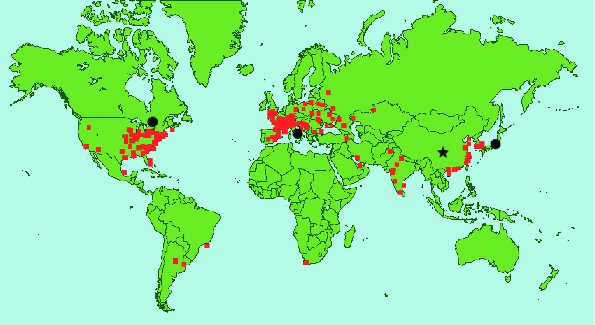
\includegraphics[width=1.0\linewidth]{img/WorldMap.jpg}
\end{figure}
\column{0.55\textwidth}
\begin{figure}
    \centering
    \caption{Total intensity of $\mu$ at different underground sites\protect\footnotemark[2]}
    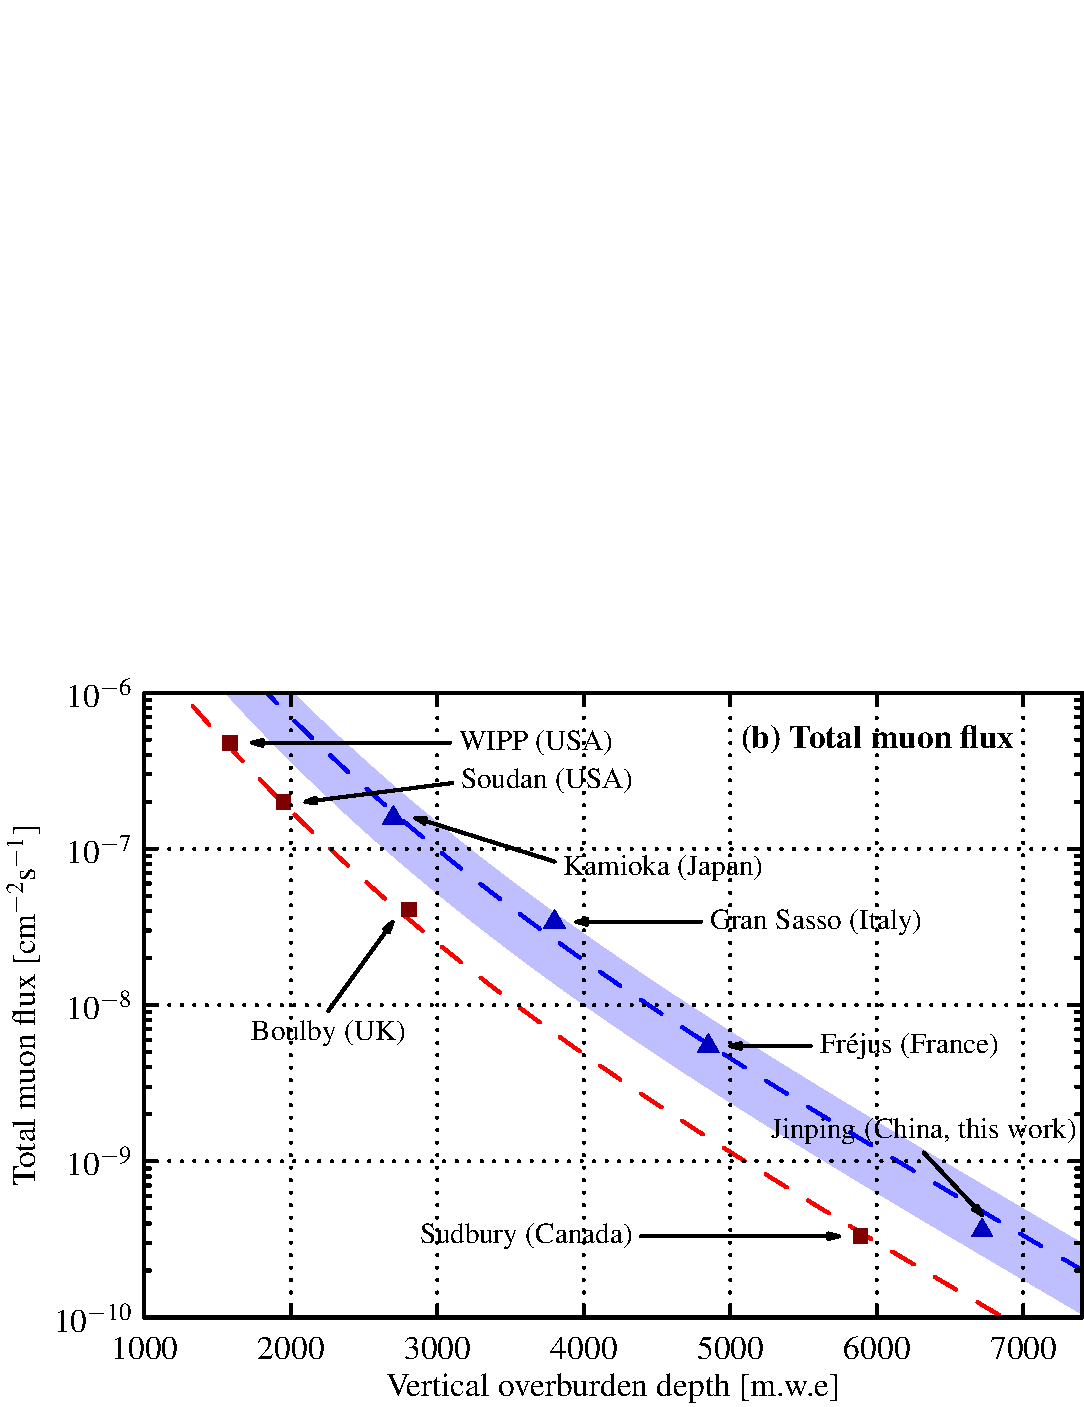
\includegraphics[width=1.0\linewidth]{img/muonlab.pdf}
\end{figure}
\end{columns}
\begin{itemize}
    \item Overburden $\sim2400\mathrm{m}$
    \item Extremely low cosmic-ray $\mu$ flux
    \item Low reactor neutrino flux
    \item Ideal site of low background physics research
\end{itemize}
\footnotetext[1]{{\tiny Beacom et al. Physics prospects of the Jinping neutrino experiment 2017}}
\footnotetext[2]{{\tiny Guo et al. Muon Flux Measurement at China Jinping Underground Laboratory 2020}}
\end{frame}

\begin{frame}
\frametitle{Jinping Neutrino Experiment}
\setlength{\abovecaptionskip}{-2mm}
\begin{figure}
    \centering
    
\includegraphics[width=0.25\linewidth]{img/J.png}
\end{figure}
\vspace{-4mm}
\begin{columns}
\column{0.33\textwidth}
\begin{center}
    Ongoing
\end{center}
\begin{figure}
    \centering
    \caption{1-ton prototype}
    \includegraphics[width=0.6\linewidth]{img/prototype.jpeg}
\end{figure}
\column{0.34\textwidth}
\begin{center}
    Next
\end{center}
\begin{figure}
    \centering
    \caption{$\sim$100t detector}
    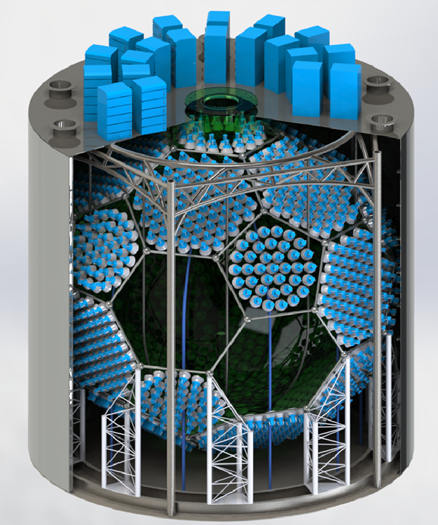
\includegraphics[width=0.6\linewidth]{img/100tondetector.png}
\end{figure}
\column{0.33\textwidth}
\begin{center}
    Future
\end{center}
\begin{figure}
    \centering
    \caption{$\sim$5000t detector}
    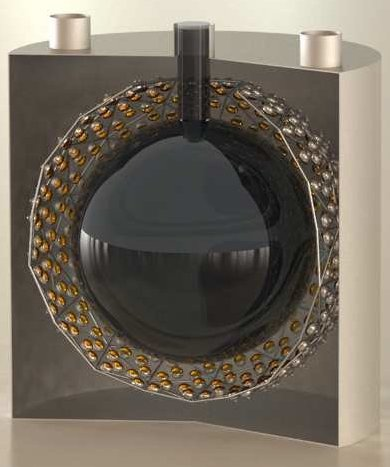
\includegraphics[width=0.6\linewidth]{img/DetectoratJinping.jpg}
\end{figure}
\end{columns}
\end{frame}

\begin{frame}
\frametitle{Neutrino Detector}
\begin{columns}
\column{0.5\textwidth}
\begin{figure}
    \centering
    \caption{Future Detector at Jinping}
    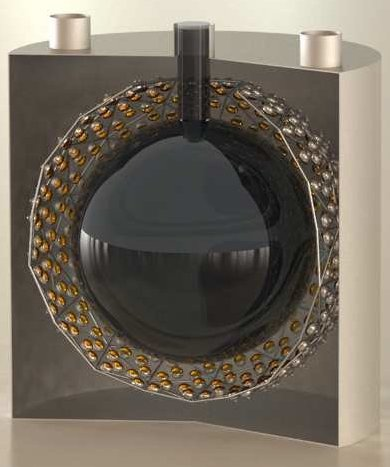
\includegraphics[width=1.0\linewidth]{img/DetectoratJinping.jpg}
\end{figure}
\column{0.5\textwidth}
\begin{itemize}
    \item Neutrino involved interaction happens in liquid scintillator produce light
    \item PMT: extremely sensitive detectors of light
    \item Timing resolution is crucial in neutrino event construction
    \item How to improve PMT's timing resolution? 
\end{itemize}
\end{columns}
\end{frame}

\begin{frame}
\frametitle{PMT timing resolution}
\setlength{\abovecaptionskip}{-2mm}
\setlength{\belowcaptionskip}{0mm}
\begin{columns}
\column{0.6\textwidth}
\begin{figure}
    \centering
    \caption{PMT}
    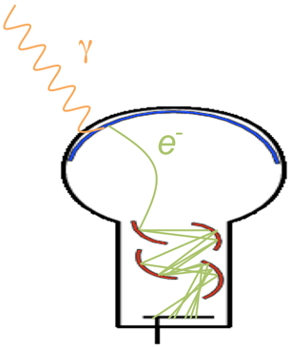
\includegraphics[width=0.25\linewidth]{img/PMT.png}
\end{figure}
\column{0.4\textwidth}
\begin{center}
    3 individual processes:
\end{center}
\vspace{-4mm}
\begin{itemize}
    \item Photon-Electron conversion
    \item Electron collection
    \item Amplify
\end{itemize}
\end{columns}
\begin{columns}
\column{0.5\textwidth}
\begin{figure}
    \centering
    \caption{PMT Single PE response}
    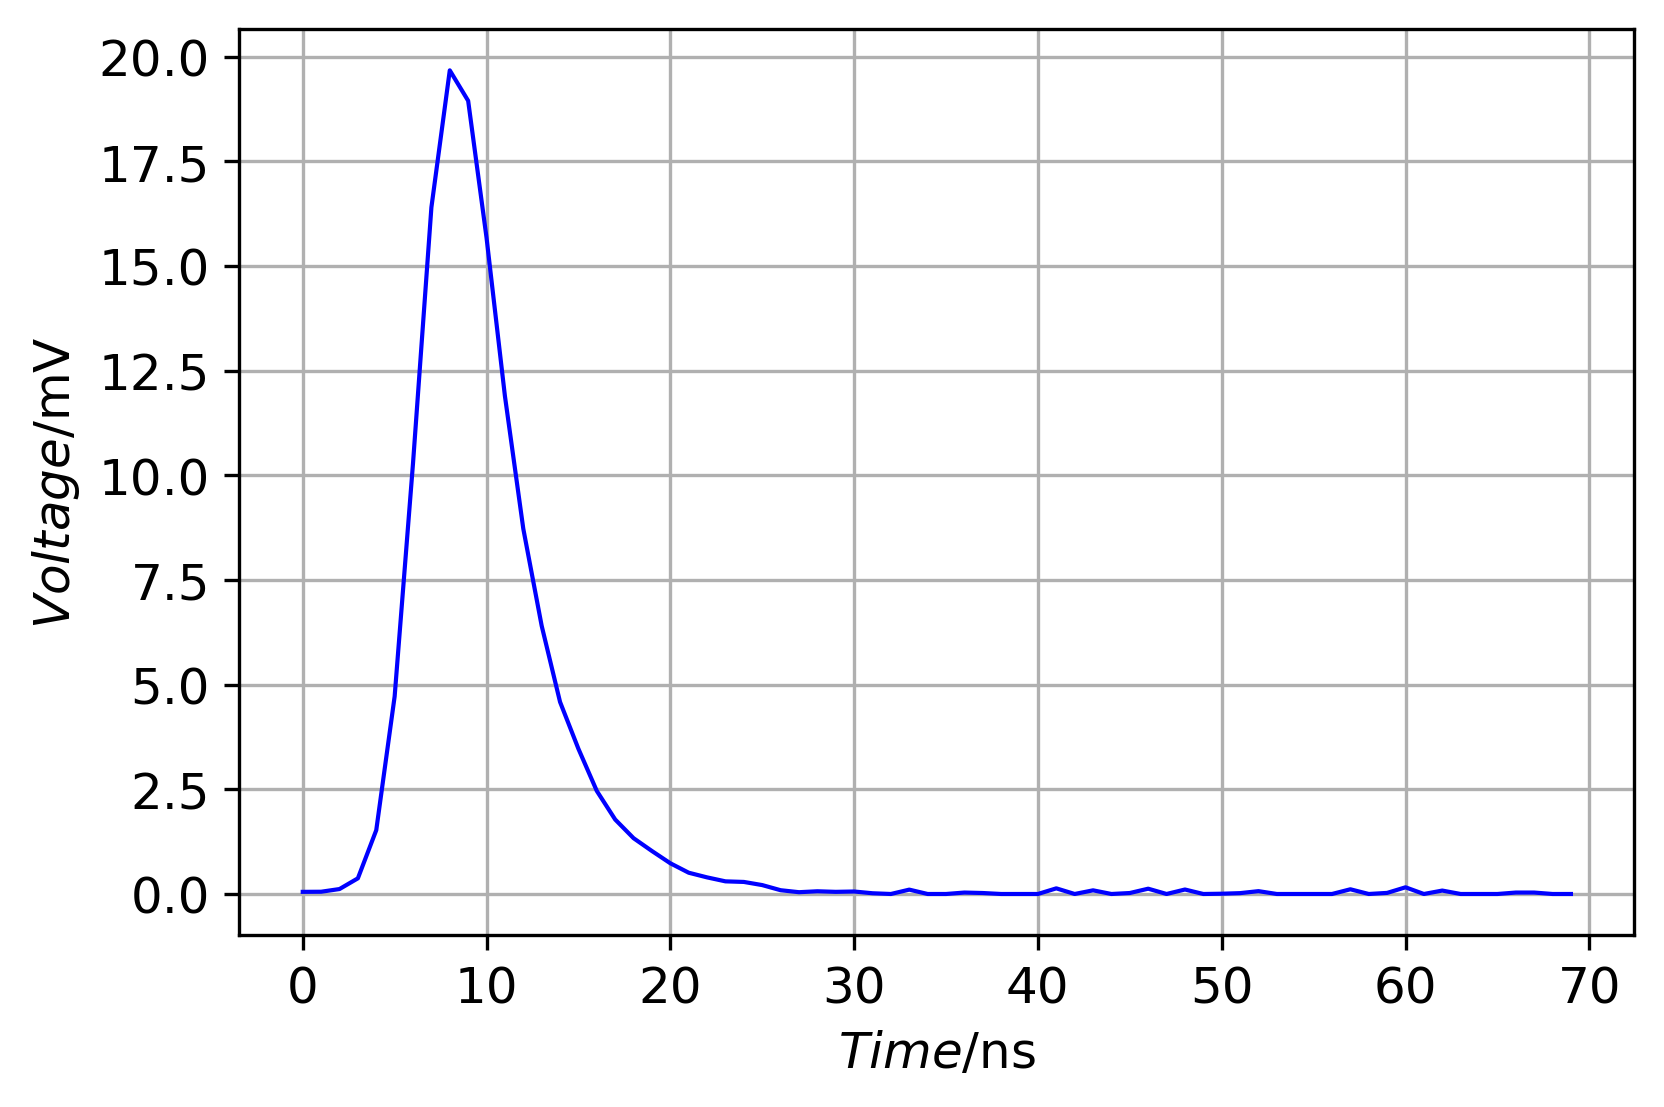
\includegraphics[width=1.0\linewidth]{img/pmtspe.png}
\end{figure}
\column{0.5\textwidth}
\begin{figure}
    \centering
    \caption{Pile-up in waveform}
    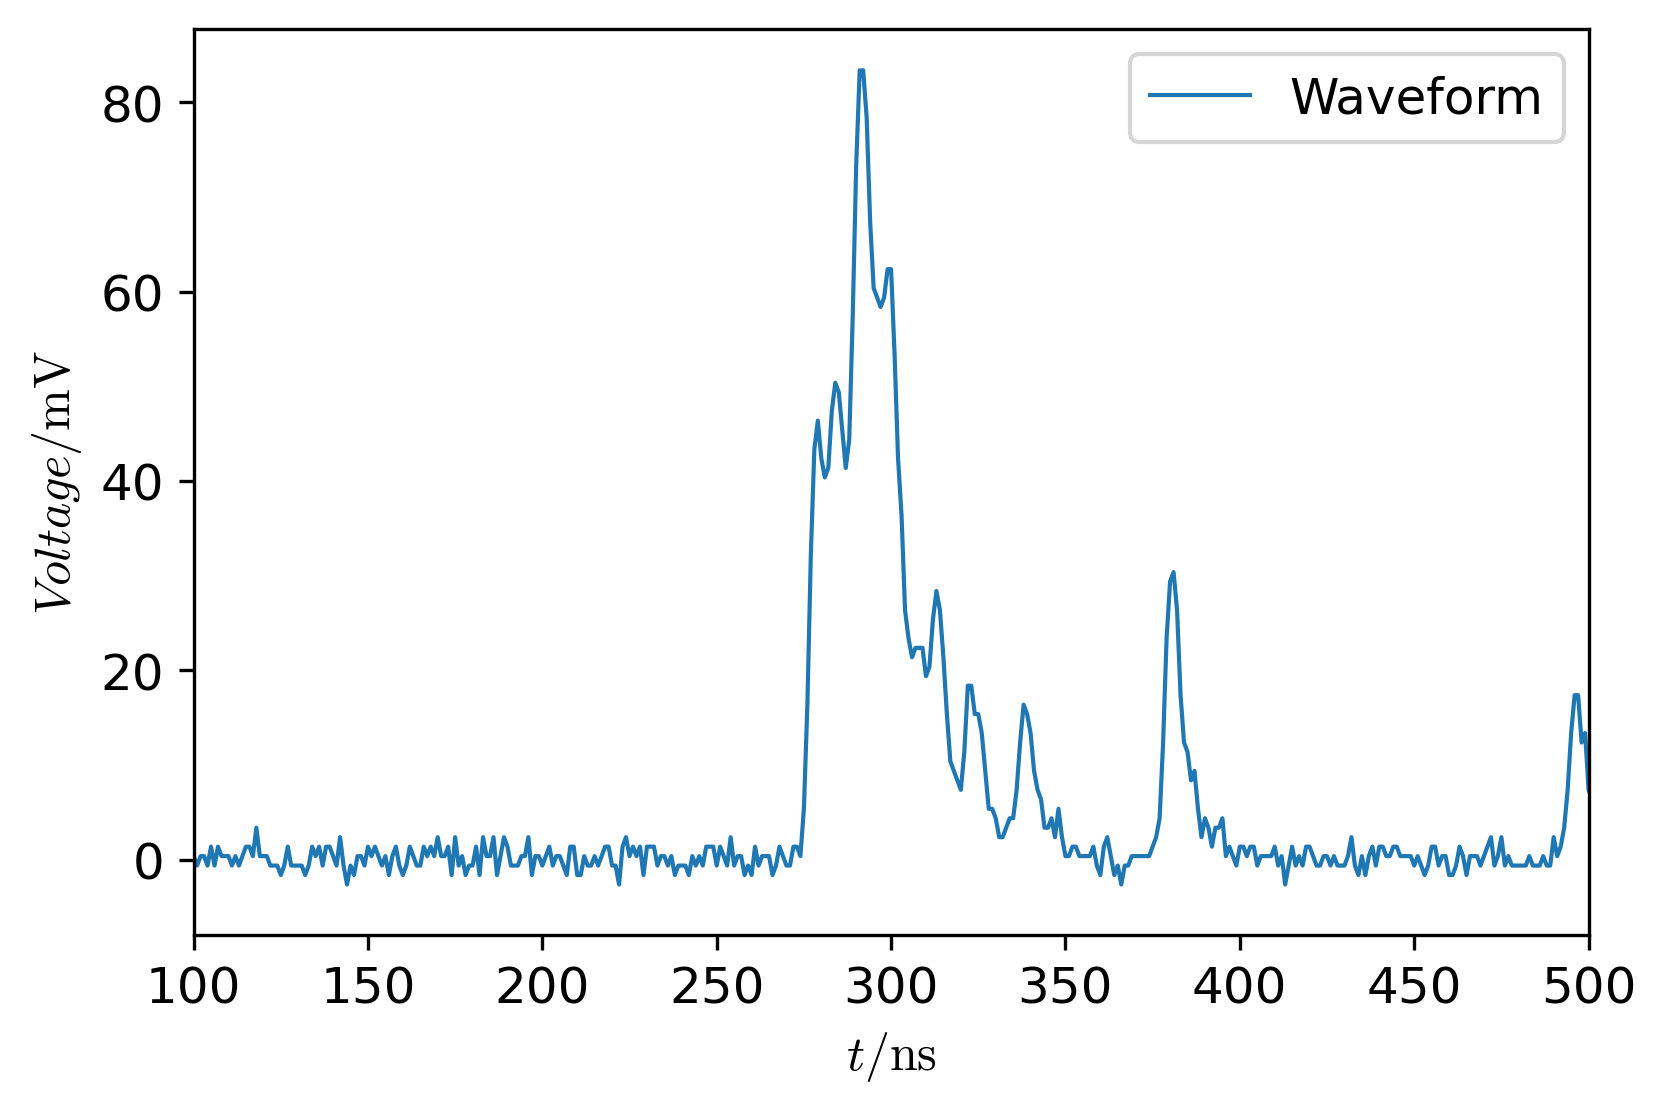
\includegraphics[width=1.0\linewidth]{img/wave.png}
\end{figure}
\end{columns}
Pile-up will significantly worsen timing resolution! 
\end{frame}

\begin{frame}
\frametitle{Naive Method to solve pile-up problem}
\hspace{4mm}Naively, when handling PMT waveforms, we record:
\begin{itemize}
    \item First HitTime
    \item Integration of Waveform (Charge)
\end{itemize}
\begin{figure}
    \centering
    % \caption{Traditional Recorded Waveform}
    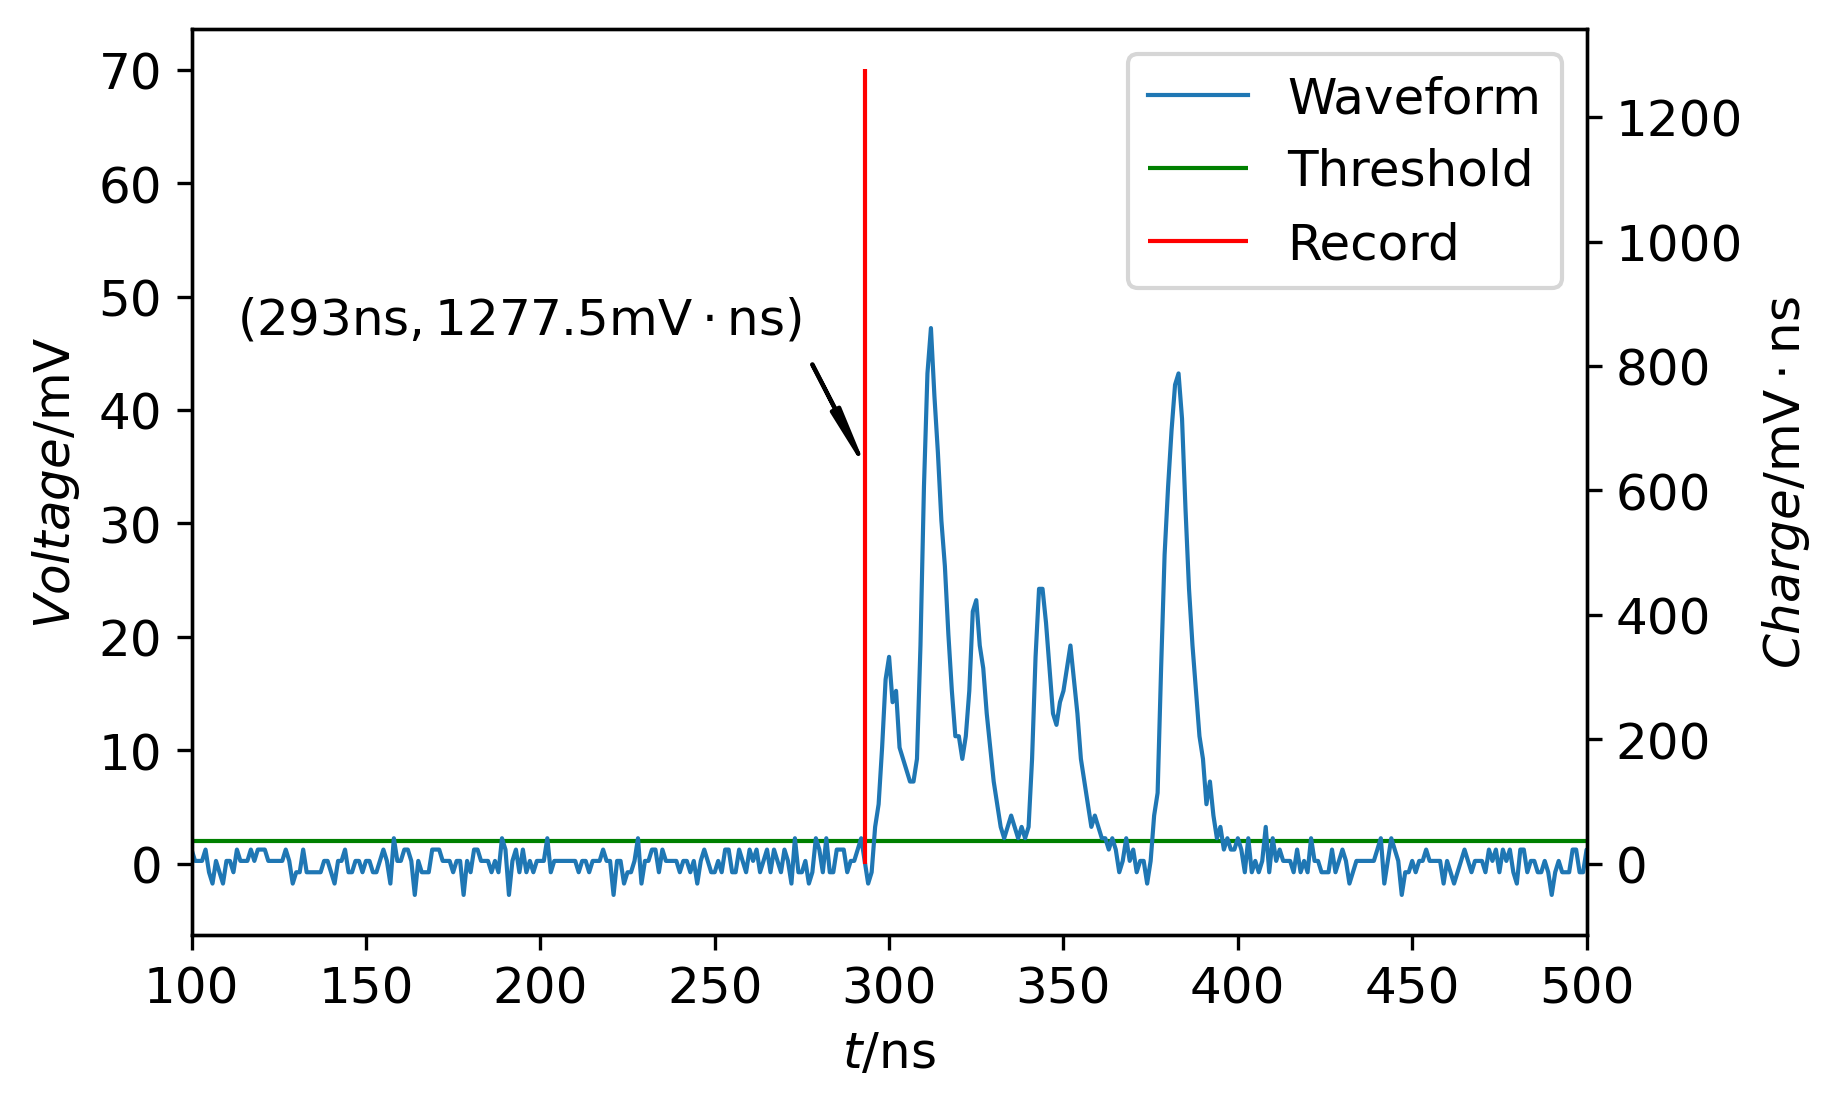
\includegraphics[width=0.8\linewidth]{img/previous.png}
\end{figure}
\end{frame}

\begin{frame}
\frametitle{New Goal to determine HitTime}
\begin{itemize}
    \item Extract All Detailed Photon Timing in 1 Window
    \item Including: HitTime (The time when electron hit first dynode) \& Charge or \#PE (number of photon electron)
\end{itemize}
\begin{figure}
    \centering
    % \caption{Traditional Recorded Waveform}
    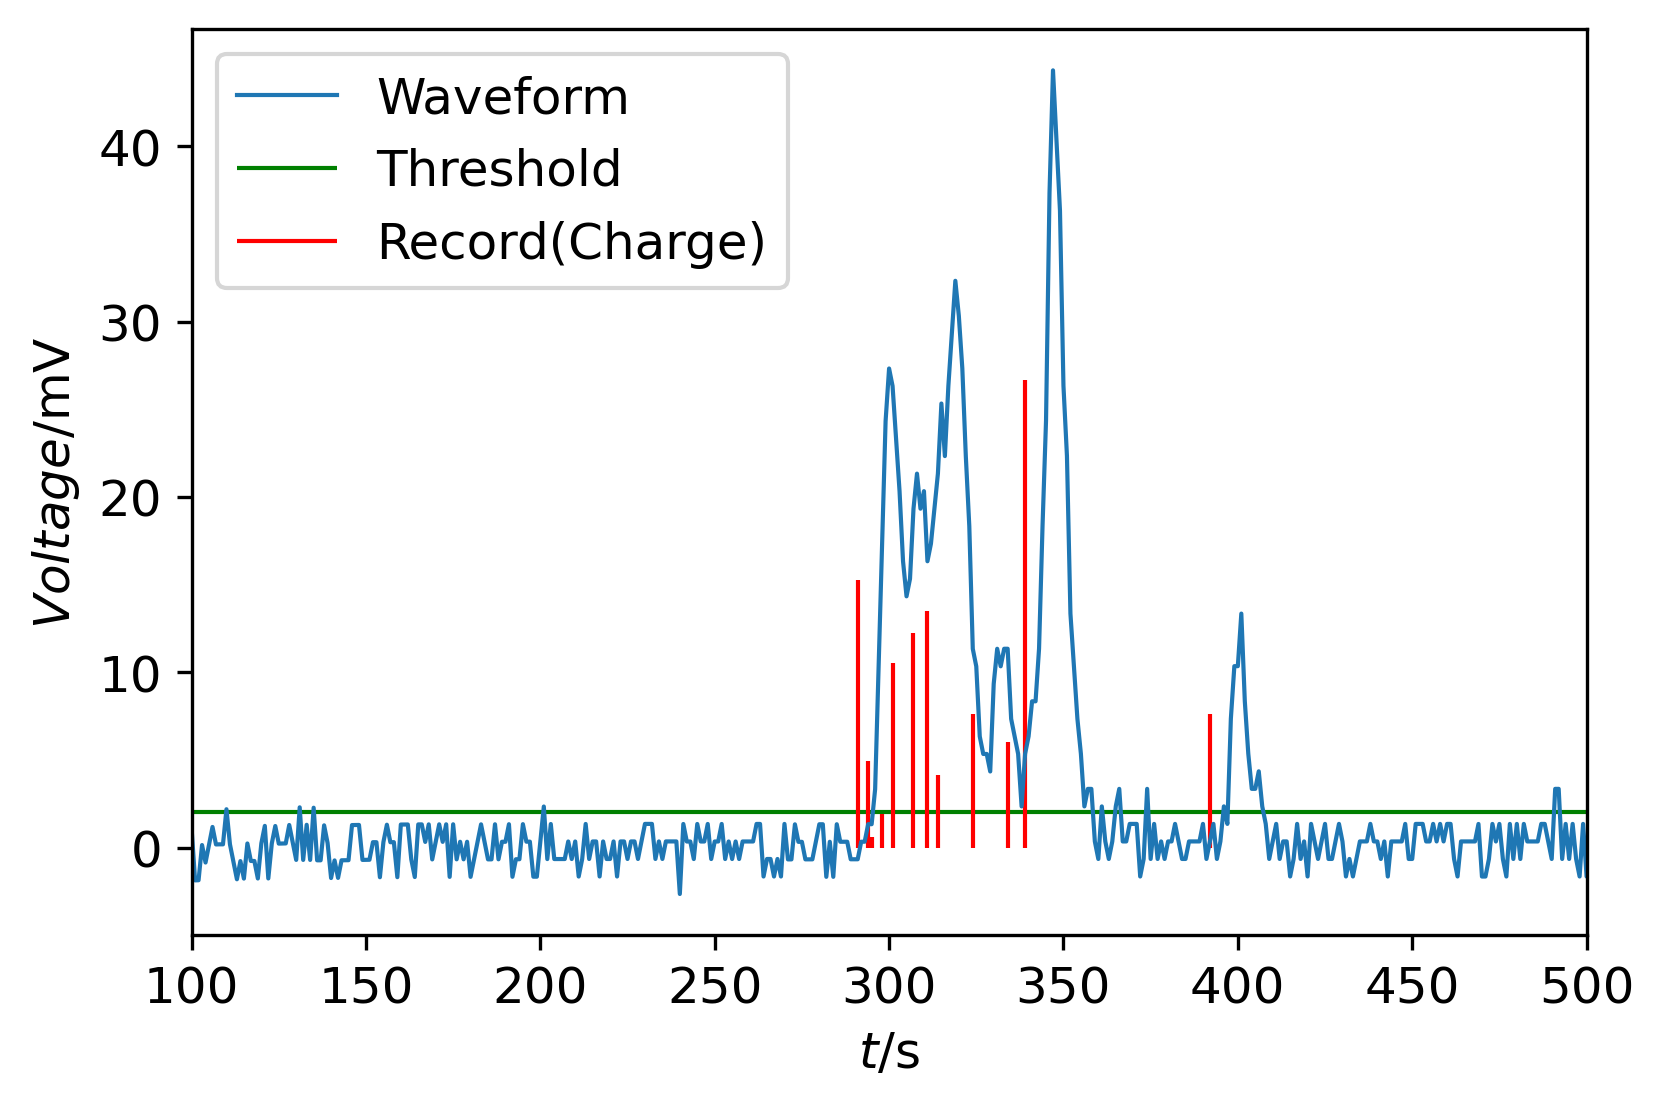
\includegraphics[width=0.8\linewidth]{img/goal.png}
\end{figure}
\end{frame}

\begin{frame}
\frametitle{Significant change of Charge for single PE}
% \setlength{\abovecaptionskip}{0mm}
% \setlength{\belowcaptionskip}{0mm}
\hspace{8mm}One PE can induce a variety of Charge
\begin{columns}
\column{0.5\textwidth}
\begin{figure}
    \centering
    \caption{10 Single PE responses}
    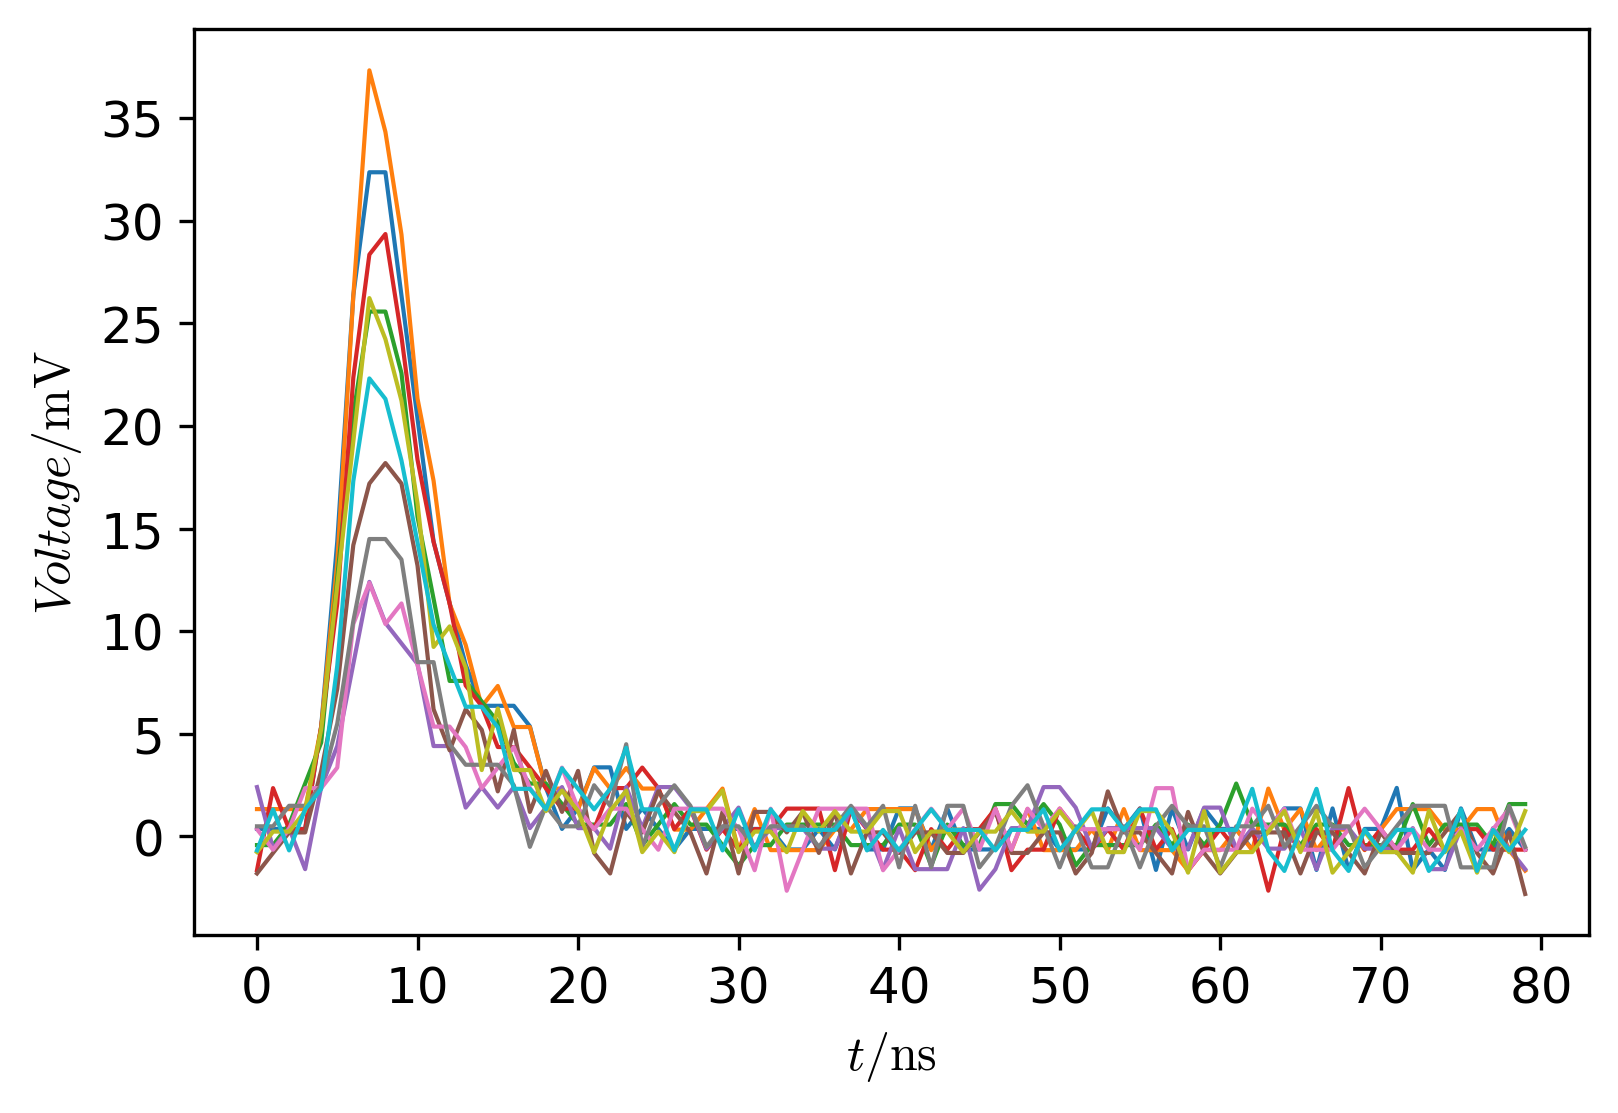
\includegraphics[width=1.0\linewidth]{img/spewaves.png}
\end{figure}
\column{0.5\textwidth}
\begin{figure}
    \centering
    \caption{Distribution of Charge}
    \includegraphics[width=1.0\linewidth]{img/chargehist.png}
\end{figure}
\end{columns}
\end{frame}

\section{Figure of merit: Wasserstein Distance}
\begin{frame}
\frametitle{The difference of Timing}
\begin{center}
    How to define the difference (distance) between reconstruction result \& truth properly?
\end{center}
\end{frame}

\begin{frame}
\frametitle{Familiar Distances}
\begin{columns}
\column{0.3\textwidth}
\begin{itemize}
    \item $L_{1}$ : $\int|p-q|$
    \item $L_{2}$ : $\int(p-q)^{2}$
    \item $\chi^{2}$ : $\int\frac{(p-q)^{2}}{q}$
    \item $\cdots$
\end{itemize}
\column{0.7\textwidth}
Shortcoming:
\begin{itemize}
    \item Cannot compare discrete distribution with continuous distribution
    \item Not sensitive to Timing
\end{itemize}
\begin{figure}
    \centering
    \includegraphics[width=1.0\linewidth]{img/tab.png}
\end{figure}
\end{columns}
\end{frame}

% % !TEX program = pdflatex
% \documentclass{beamer}

% % \usetheme{Madrid}
% \usepackage{amsmath,mathrsfs}
% \usepackage{tikz}

\tikzset{elegant/.style={smooth,thick,samples=50,cyan}}
\tikzset{eaxis/.style={->,>=stealth}}

% \begin{document}
\begin{frame}
    \frametitle{Wasserstein Distance}
    \resizebox{\textwidth}{!}{
    \begin{tikzpicture}
        % draw the axis
        \draw[eaxis] (-1.5,0) -- (4,0);
        % draw the function (piecewise)
        \draw[elegant,domain=-1.5:3.5] plot(\x,{pow(e,-(\x)^2*4)*2}) node [anchor=east] at (0,2) {$\mu(a)$};
        \draw[elegant,orange,domain=-1.5:3.5] plot(\x,{pow(e,-(\x-1)^2)}) node [anchor=west] at (1.1,1.1) {$\nu(b)$};
        
        \draw[->] (0,2) to[out=0, in=90] (1,1);
        \node at (1.4,1.9)  {\tiny$W(\mu(a),\nu(b))$};
    \end{tikzpicture}
    }
    \begin{center}
        Minimal effort transporting mass form $\mu$ to $\nu$
    \end{center}
\end{frame}
\begin{frame}
    \frametitle{Wasserstein Distance}
    \resizebox{\textwidth}{!}{
    \begin{tikzpicture}
        % draw the axis
        \draw[eaxis] (-1.5,0) -- (4,0);
        % draw the function (piecewise)
        \draw[elegant,domain=-1.5:3.5] plot(\x,{pow(e,-(\x)^2*4)*2});
        \draw[elegant,orange,domain=-1.5:3.5] plot(\x,{pow(e,-(\x-1)^2)});
        
        \draw[fill=red] (-0.15,0.3) rectangle (-0.05,0.9) node [anchor=east] (block1) {};
        \draw[fill=green] (-0.15,0.9) rectangle (-0.05,1.9) node [anchor=east] (block2) {};
        \draw[fill=red] (0.65,0.3) rectangle (0.75,0.9) node (block3) {};
        \draw[fill=green] (0.85,0.09) rectangle (0.95,0.99) node (block4) {};
        
        \draw (-0.1,0.3) -- (-0.1,0) node [anchor=north] {\tiny$a$};
        \draw (0.7,0.3) -- (0.7,0) node [anchor=north] {\tiny$b_1$};
        \draw (0.9,0.1) -- (0.9,0) node [anchor=north] {\tiny$b_2$};
        
        \draw[red,->] (block1) -- (block3);
        \draw[green,->] (block2) to[out=0, in=120] (block4);
    \end{tikzpicture}
    }
    \begin{center}
        the transport plan from $a$ to $b$ is described by $\pi(a, b)$
    \end{center}
\end{frame}

\begin{frame}
    \frametitle{Wasserstein Distance}
    \resizebox{\textwidth}{!}{
    \begin{tikzpicture}
        % draw the axis
        \draw[eaxis] (-1.5,0) -- (4,0);
        % draw the function (piecewise)
        \draw[elegant,domain=-1.5:3.5] plot(\x,{pow(e,-(\x)^2*4)*2});
        \draw[elegant,orange,domain=-1.5:3.5] plot(\x,{pow(e,-(\x-1)^2)});
        
        \draw[fill=red] (-0.15,0.3) rectangle (-0.05,0.9) node [anchor=east] (block1) {};
        \draw[<->] (-0.2,0.3) -- (-0.2,0.9);
        \node [anchor=east] at (-0.1,0.6) {\tiny$\pi(a,b_1)\Delta b_1$};
        \draw[fill=green] (-0.15,0.9) rectangle (-0.05,1.9) node [anchor=east] (block2) {};
        \draw[<->] (-0.2,0.9) -- (-0.2,1.9);
        \node [anchor=east] at (-0.1,1.4) {\tiny$\pi(a,b_2)\Delta b_2$};
        \draw[fill=red] (0.65,0.3) rectangle (0.75,0.9) node (block3) {};
        \draw[fill=green] (0.85,0.09) rectangle (0.95,0.99) node (block4) {};
        
        \draw (-0.1,0.3) -- (-0.1,0) node [anchor=north] {\tiny$a$};
        \draw (0.7,0.3) -- (0.7,0) node [anchor=north] {\tiny$b_1$};
        \draw (0.9,0.1) -- (0.9,0) node [anchor=north] {\tiny$b_2$};
        
        \draw[red,->] (block1) -- (block3);
        \node at (0.38,1.05)  {\tiny$d(a,b_1)$};
        \draw[green,->] (block2) to[out=0, in=120] (block4);
        \node at (0.6,1.6)  {\tiny$d(a,b_2)$};
    \end{tikzpicture}
    }
\begin{equation*}
    \begin{aligned}
        &mass: \pi(a,b)\Delta a\Delta b \ \ \  path: d(a, b) \\
        &\Delta W={\color{red}\pi(a,b_1)\Delta a\Delta b_1}d(a,b_1) + {\color{green}\pi(a,b_2)\Delta a\Delta b_2}d(a,b_2) \\
    \end{aligned}
\end{equation*}
\pause
\begin{equation*}
    \begin{aligned}
        \hspace{-4mm}&W(\mu(a),\nu(b))|_{\pi=\pi(a,b)} = \iint \pi(a,b)d(a,b)\mathrm{d}a\mathrm{d}b = \int d(a,b)\mathrm{d}\pi(a,b)\\
    \end{aligned}
\end{equation*}
\end{frame}
\begin{frame}
    \frametitle{Wasserstein Distance}
    \resizebox{\textwidth}{!}{
    \begin{tikzpicture}
        % draw the axis
        \draw[eaxis] (-1.5,0) -- (4,0);
        % draw the function (piecewise)
        \draw[elegant,domain=-1.5:3.5] plot(\x,{pow(e,-(\x)^2*4)*2});
        \draw[elegant,orange,domain=-1.5:3.5] plot(\x,{pow(e,-(\x-1)^2)});
        
        \draw[fill=red] (-0.15,0.3) rectangle (-0.05,0.9) node [anchor=east] (block1) {};
        \draw[<->] (-0.2,0.3) -- (-0.2,0.9);
        \node [anchor=east] at (-0.1,0.6) {\tiny$\pi(a,b_1)\Delta b_1$};
        \draw[fill=green] (-0.15,0.9) rectangle (-0.05,1.9) node [anchor=east] (block2) {};
        \draw[<->] (-0.2,0.9) -- (-0.2,1.9);
        \node [anchor=east] at (-0.1,1.4) {\tiny$\pi(a,b_2)\Delta b_2$};
        \draw[fill=red] (0.65,0.3) rectangle (0.75,0.9) node (block3) {};
        \draw[fill=green] (0.85,0.09) rectangle (0.95,0.99) node (block4) {};
        
        \draw (-0.1,0.3) -- (-0.1,0) node [anchor=north] {\tiny$a$};
        \draw (0.7,0.3) -- (0.7,0) node [anchor=north] {\tiny$b_1$};
        \draw (0.9,0.1) -- (0.9,0) node [anchor=north] {\tiny$b_2$};
        
        \draw[red,->] (block1) -- (block3);
        \node at (0.38,1.05)  {\tiny$d(a,b_1)$};
        \draw[green,->] (block2) to[out=0, in=120] (block4);
        \node at (0.6,1.6)  {\tiny$d(a,b_2)$};
    \end{tikzpicture}
    }
    Choosing the best transportaion $\pi(a,b) \in \Pi(\mu,\nu)$:
\begin{equation*}
    \begin{aligned}
        \mathrm{Wasserstein}(\mu(a),\nu(b)) &= \inf_{\pi \in \Pi(\mu,\nu)} W(\mu(a),\nu(b))|_{\pi=\pi(a,b)} \\
        &=\inf_{\pi \in \Pi(\mu,\nu)}\int d(a,b)\mathrm{d}\pi(a,b)\\
    \end{aligned}
\end{equation*}
\end{frame}   
% \end{document}
%         % 建立相对坐标系
%         % \draw[help lines,xstep=.1,ystep=.1] (-1.5,0) grid (pi,2);

\begin{frame}
\frametitle{Wasserstein Distance Demo}
\setlength{\abovecaptionskip}{-2mm}
\setlength{\belowcaptionskip}{0mm}
$D_{w}=\sum|\mathrm{CDF}(a) - \mathrm{CDF}(b)|$ \\
$CDF$: Cumulative Distribution Function
\begin{columns}
\column{0.4\textwidth}
\begin{figure}
    \centering
    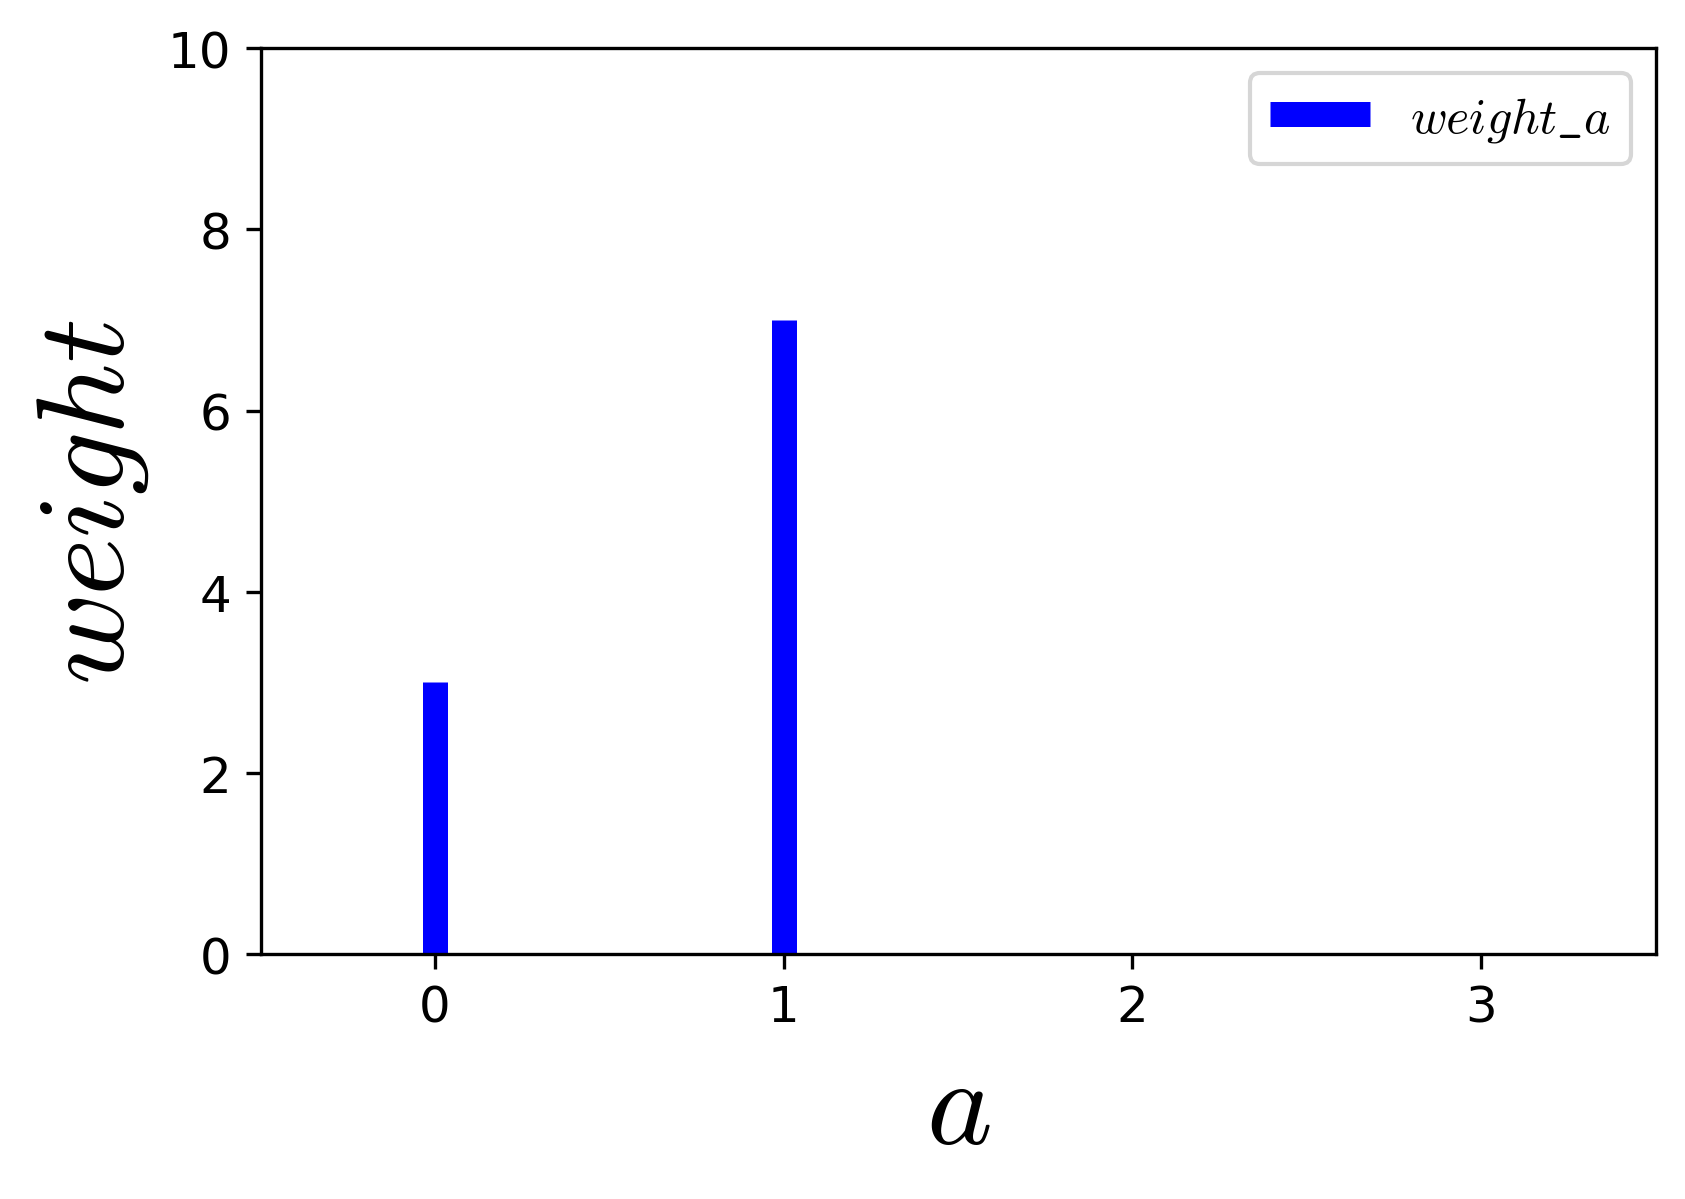
\includegraphics[width=1.0\linewidth]{img/a.png}
\end{figure}
\vspace{-7mm}
\begin{figure}
    \centering
    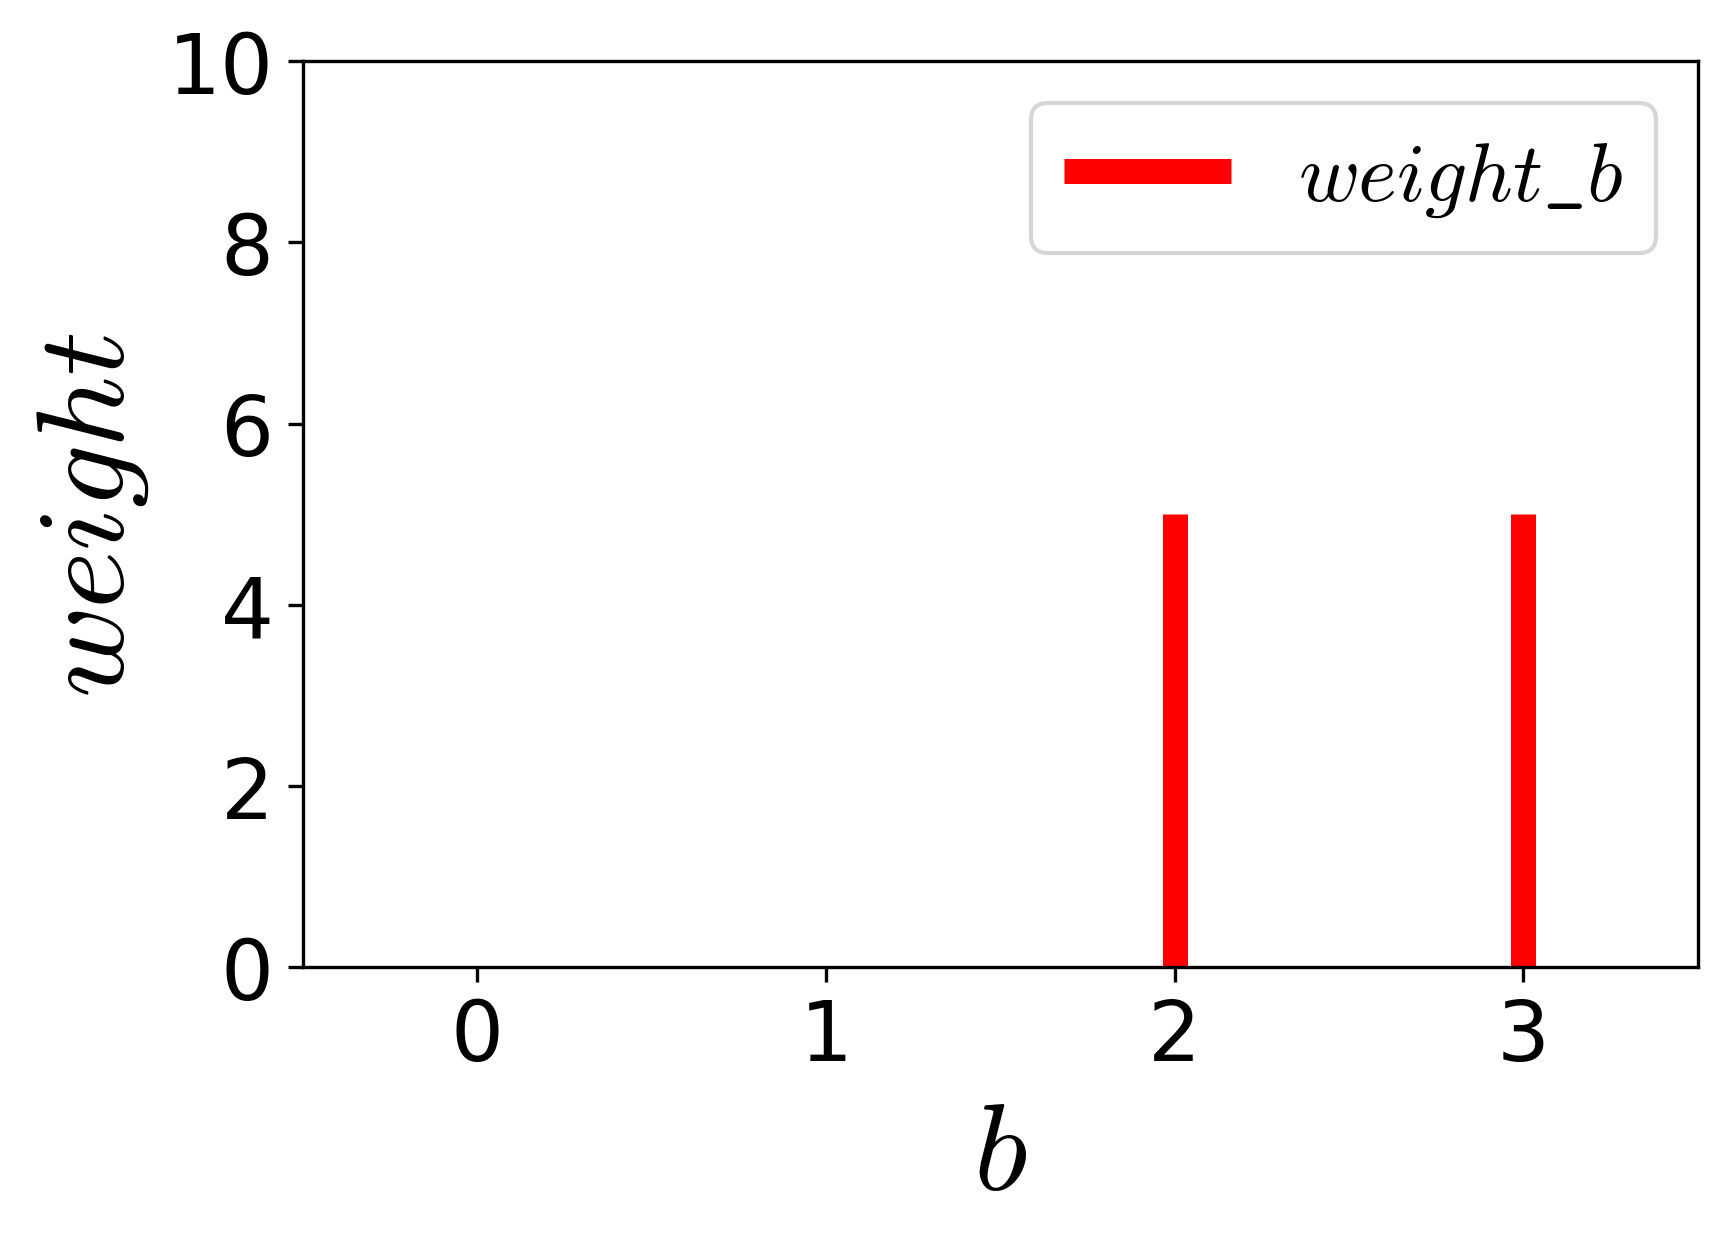
\includegraphics[width=1.0\linewidth]{img/b.png}
\end{figure}
\column{0.1\textwidth}
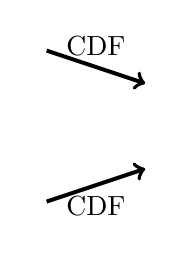
\begin{tikzpicture}
    \node[] at (-2.5, 1) (a1) {};
    \node[] at (-1, 0.5) (a2) {};
    \node[] at (-2.5, -1) (b1) {};
    \node[] at (-1, -0.5) (b2) {};
    \draw [->, line width=0.5mm] (a1) -- node[anchor=south] {CDF} (a2);
    \draw [->, line width=0.5mm] (b1) -- node[anchor=north] {CDF} (b2);
\end{tikzpicture}
\column{0.5\textwidth}
\vspace{2mm}\begin{figure}
    \centering
    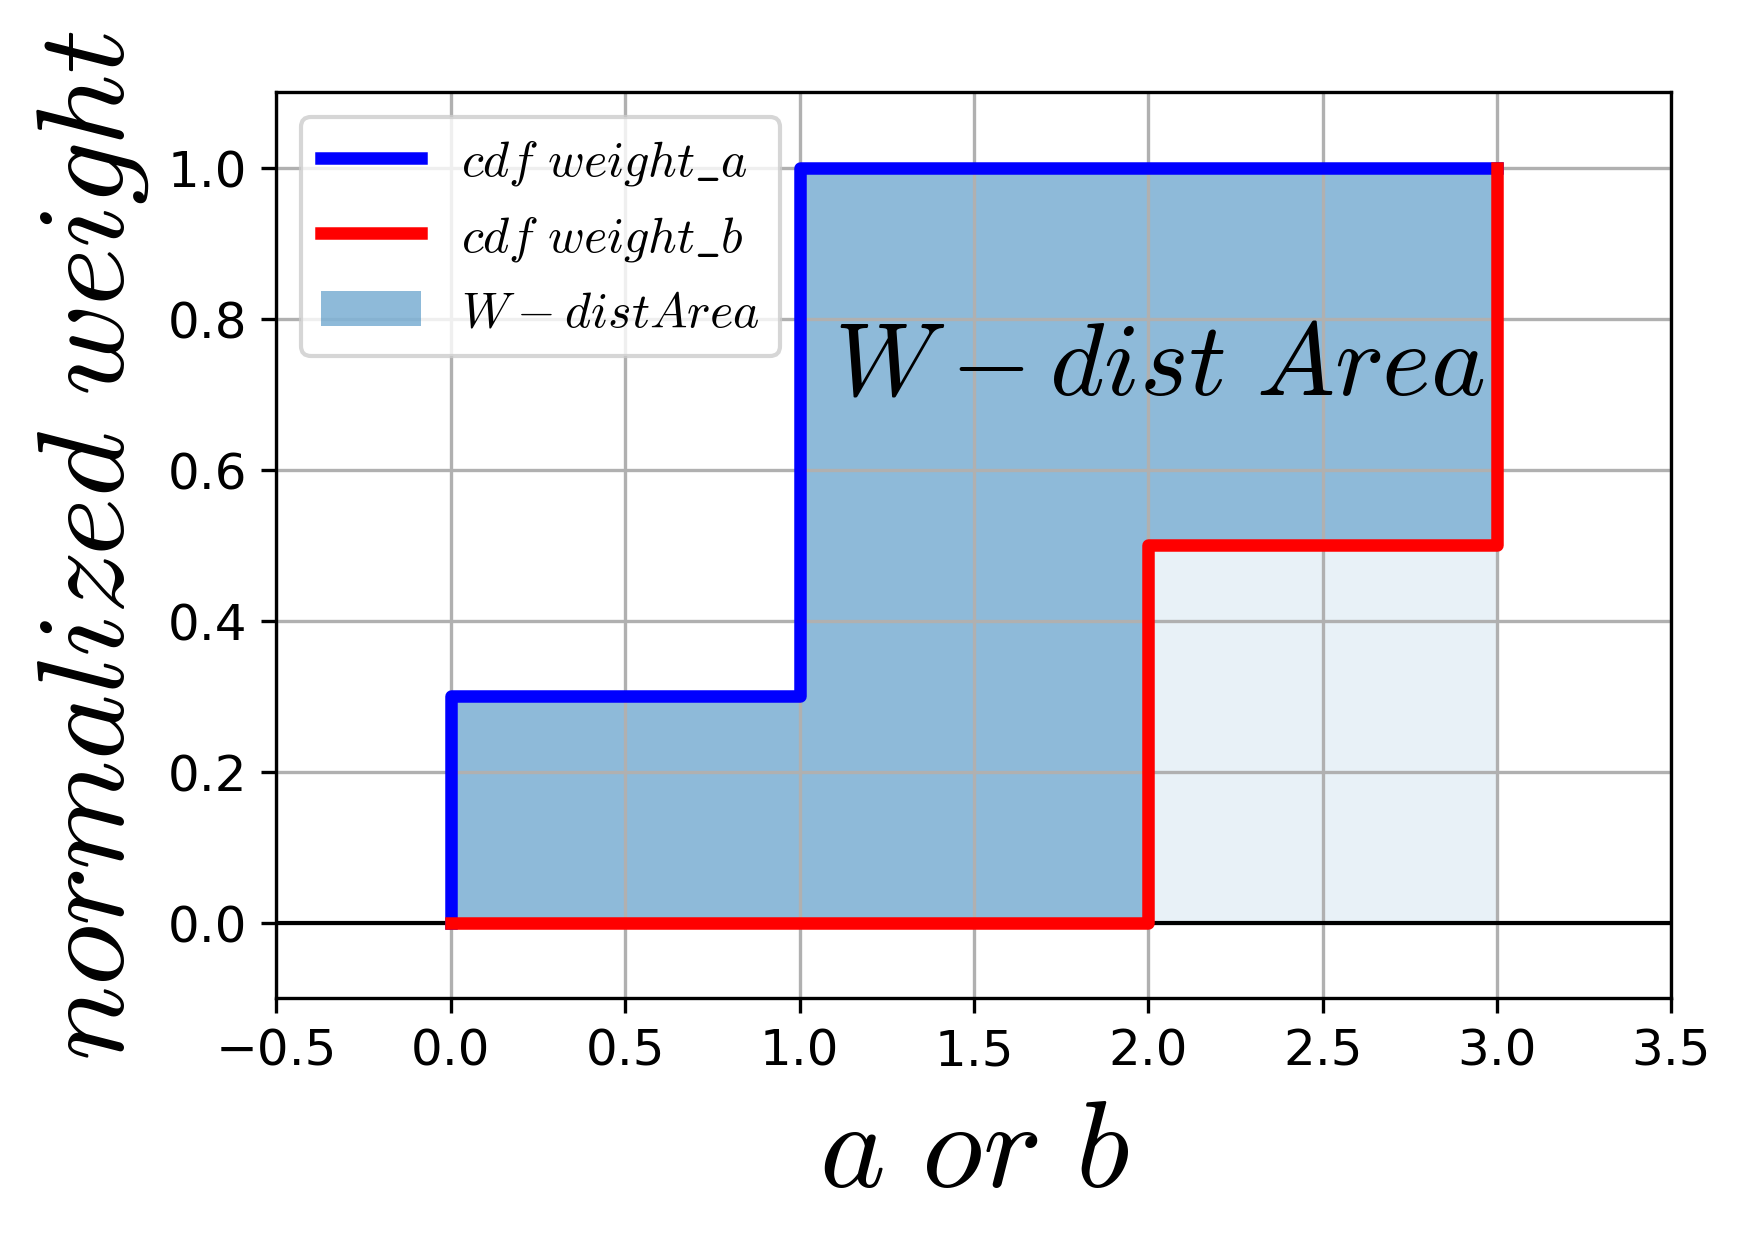
\includegraphics[width=1.0\linewidth]{img/ab.png}
\end{figure}
\rightline{W-dist = $1.8\mathrm{ns}$}
\end{columns}
This definition of distance is equivalent to Wasserstein Distance
\end{frame}

\section{Waveform Analysis Methods}

\begin{frame}
\frametitle{Test Setup}
\begin{columns}
\column{0.4\textwidth}
\hspace{4mm}Input \& Output:
\begin{itemize}
    \item Input: Pedestal subtracted PMT waveform
    \item Output: Weight (Charge or \#PE) sequence
\end{itemize}
\hspace{4mm}Loss:

\hspace{4mm}Wasserstein distance \\ \hspace{4mm}between reconstruction \\ \hspace{4mm}result \& truth
\column{0.6\textwidth}
\setlength{\abovecaptionskip}{-2mm}
\setlength{\belowcaptionskip}{0mm}
\begin{figure}
    \centering
    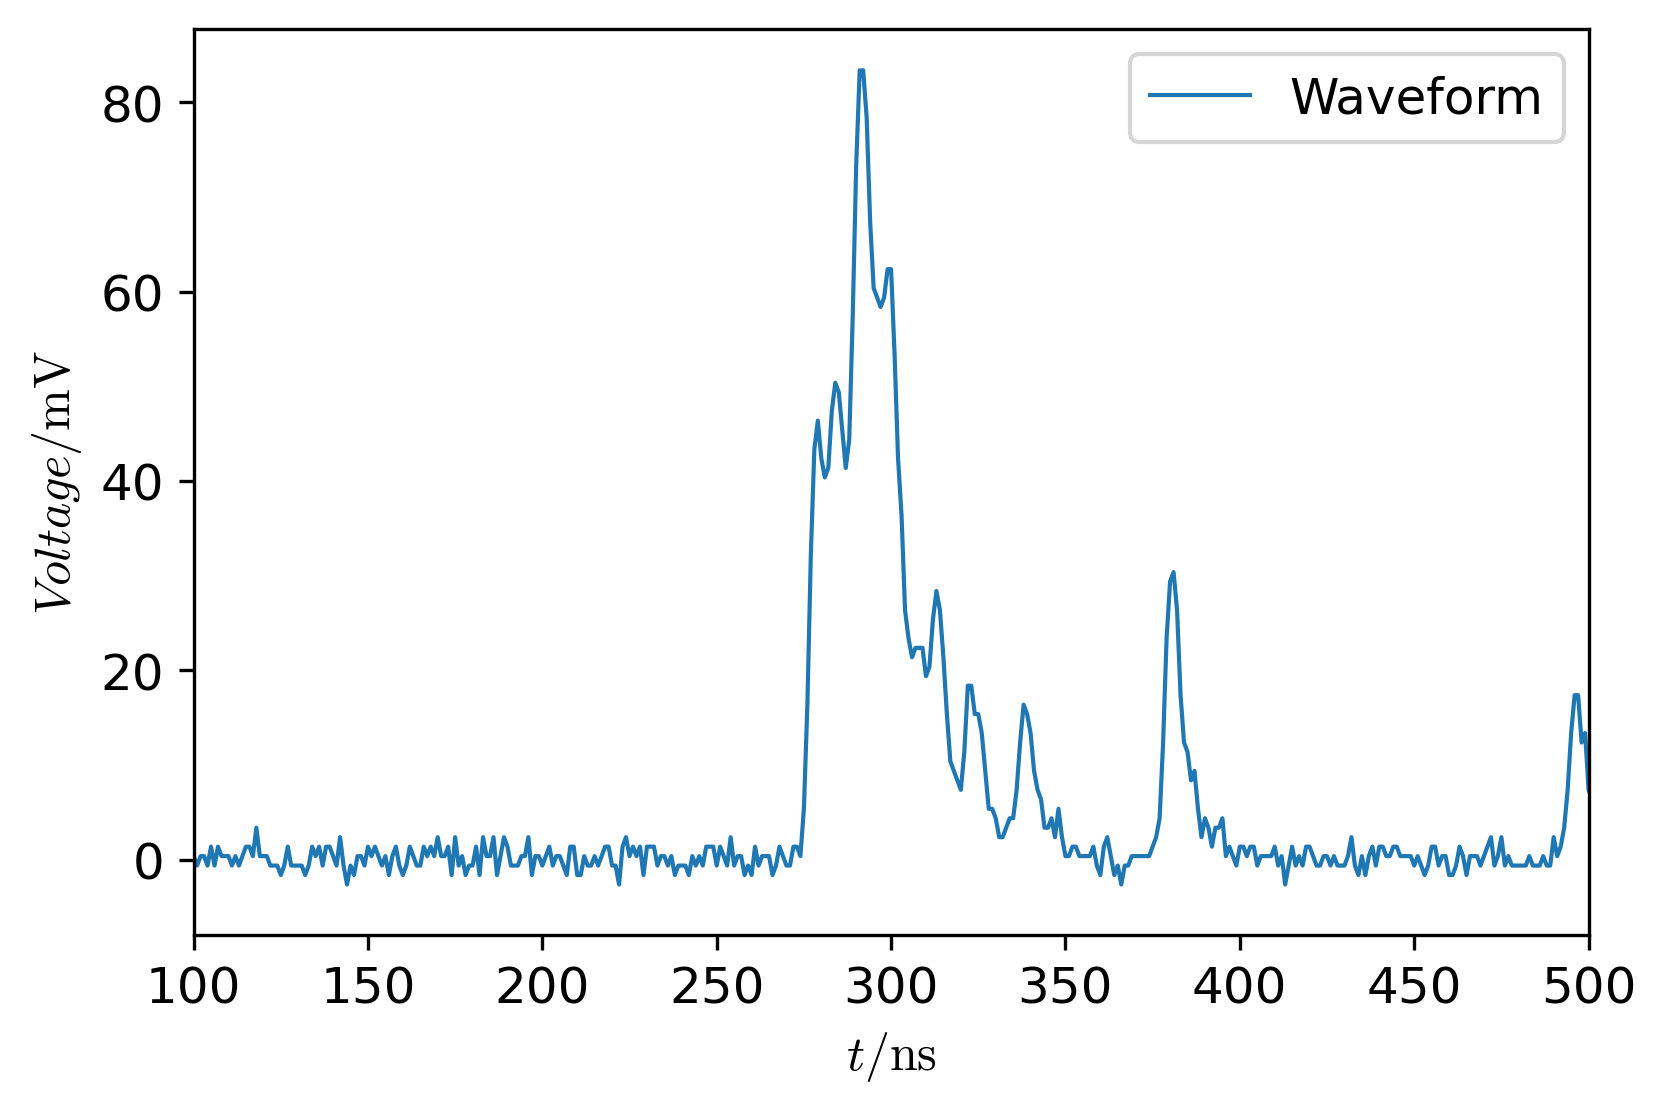
\includegraphics[width=0.9\linewidth]{img/wave.png}
    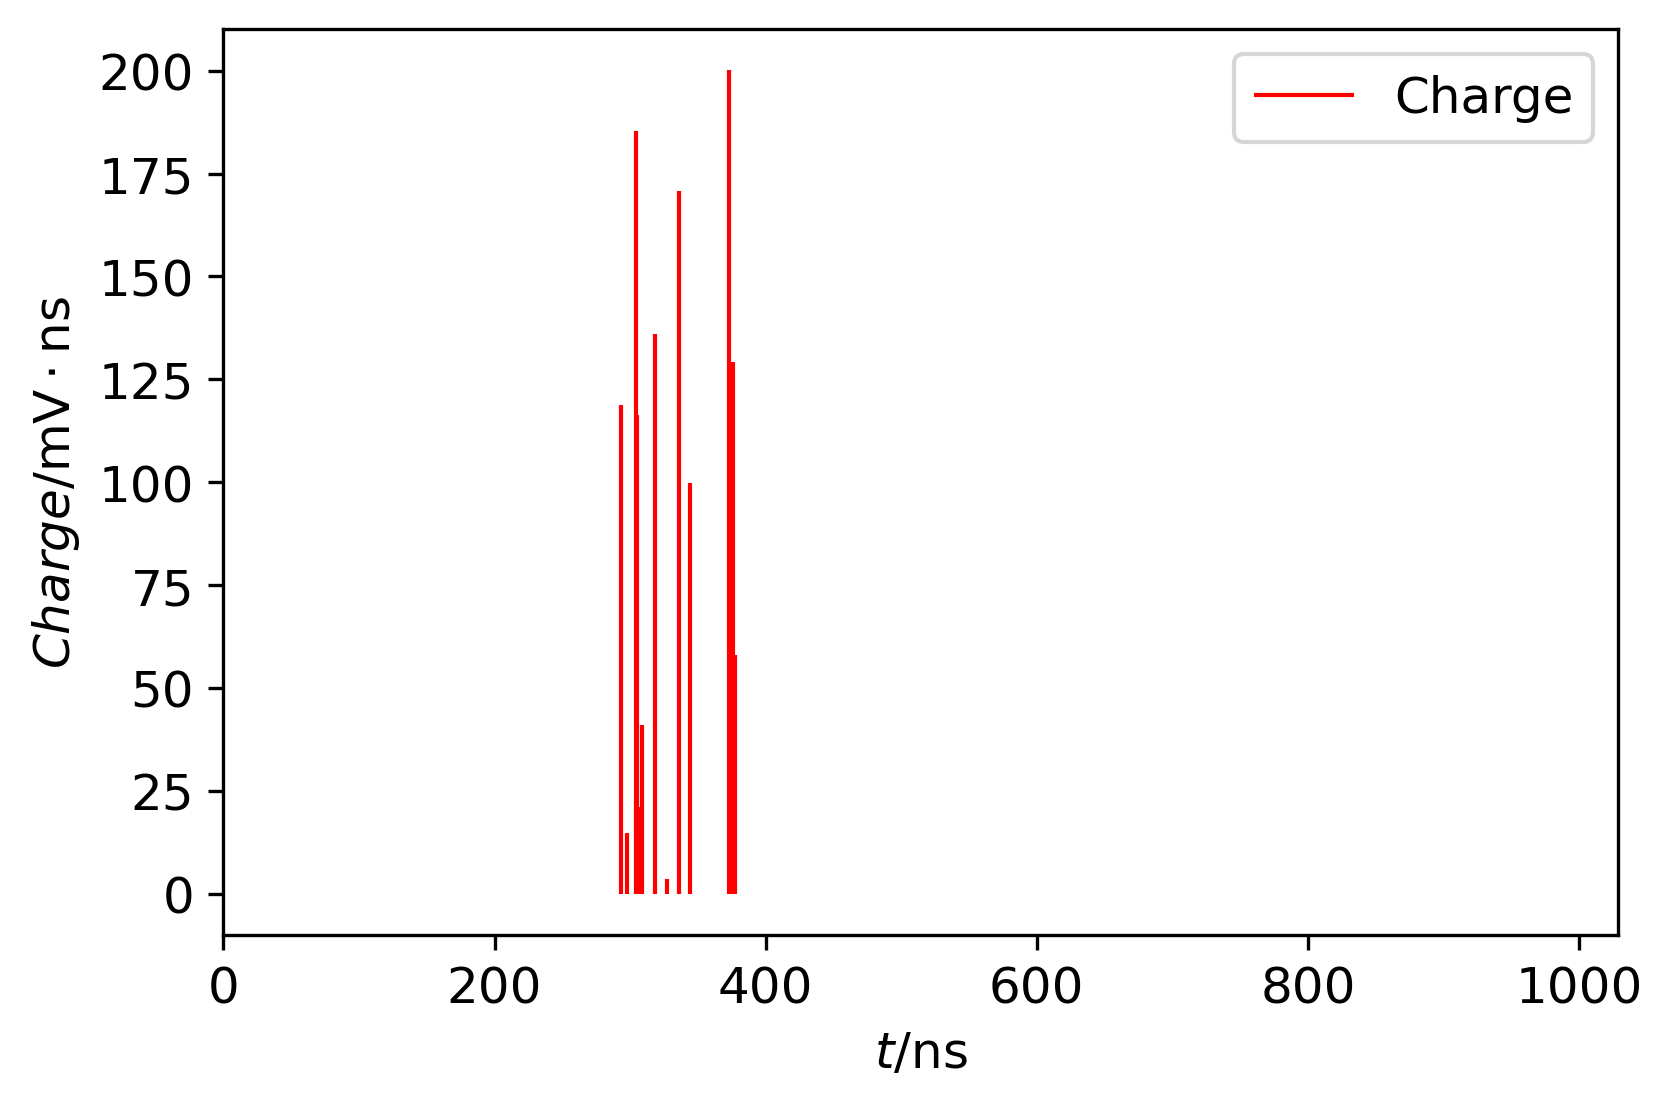
\includegraphics[width=0.9\linewidth]{img/charge.png}
\end{figure}
\end{columns}
\end{frame}

\begin{frame}
\frametitle{Data Sample}
TotalPEnum is the count of HitTime in one waveform
\begin{columns}
\column{0.6\textwidth}
\begin{figure}
    \centering
    \caption{TotalPEnum Histogram}
    \includegraphics[width=1.0\linewidth]{img/penum.png}
\end{figure}
\column{0.4\textwidth}
\begin{figure}
    \centering
    \caption{Data Structure}
    \includegraphics[width=1.0\linewidth]{img/dataset.png}
\end{figure}
\end{columns}
\end{frame}

\begin{frame}
\frametitle{Method 1: Find Peak}
\begin{figure}
    \centering
    \caption{Find Peak Method Demo, W-dist = 4.02}
    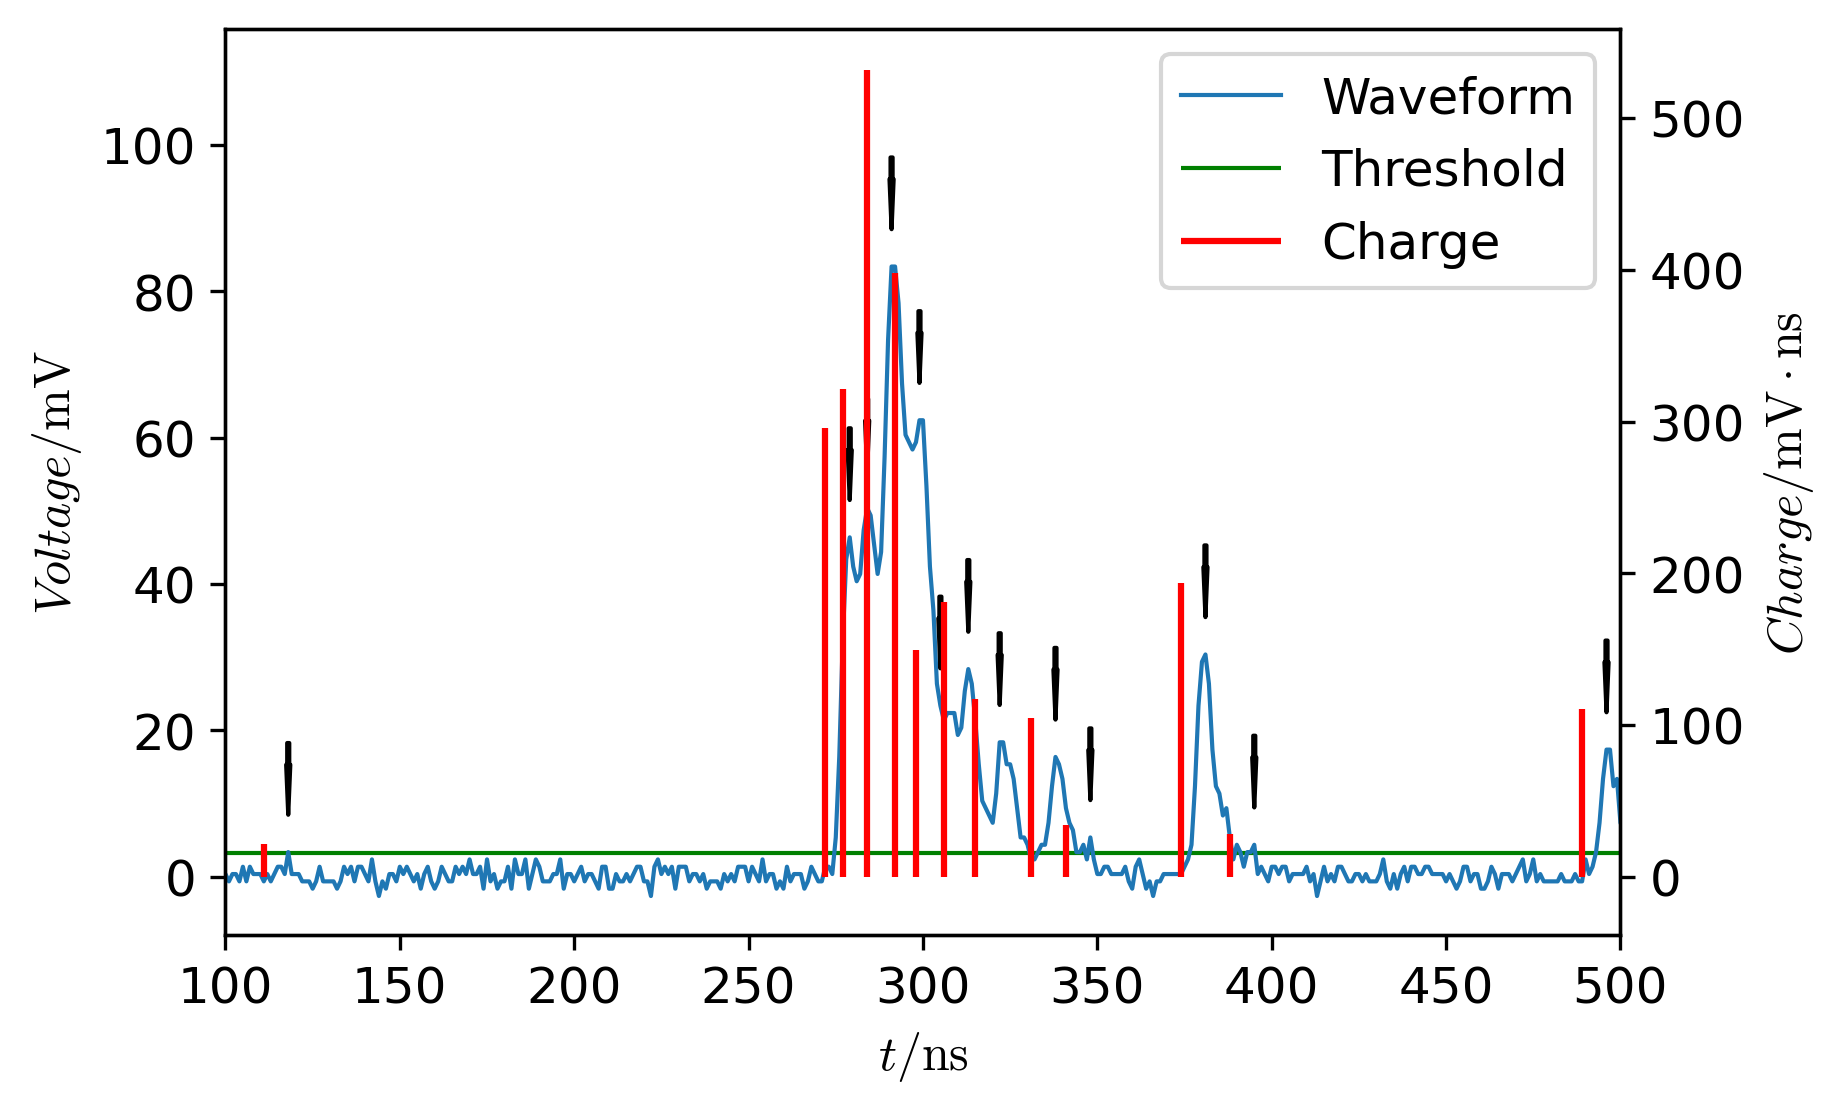
\includegraphics[width=0.9\linewidth]{img/findpeak.png}
\end{figure}
\vspace{-4mm}
\begin{center}
    Average W-dist = 10.70 (Charge), 11.62 (\#PE)
\end{center}
\end{frame}

\begin{frame}
\frametitle{Method 2: Waveform Shift}
\begin{figure}
    \centering
    \caption{Waveform Shift Method Demo, W-dist = 10.75}
    \includegraphics[width=0.9\linewidth]{img/threshold.png}
\end{figure}
\vspace{-4mm}
\begin{center}
    Average W-dist = 3.67 (Charge), 4.69 (\#PE)
\end{center}
\end{frame}

\begin{frame}
\frametitle{Method 3: Fourier Deconvolution}
\begin{columns}
\column{0.6\textwidth}
\begin{figure}
    \centering
    \caption{Fourier Deconvolution Demo, W-dist = 1.63}
    \includegraphics[width=1.0\linewidth]{img/fftrans.png}
\end{figure}
\vspace{-4mm}
\begin{center}
    Average W-dist = 1.44 (Charge), 3.08 (\#PE)
\end{center}
\column{0.4\textwidth}
\begin{enumerate}
    \item FFT of Waveform \& Single PE response
    \item Rectangular filter of FFT(Waveform)
    \item FFT(Charge) = FFT(Waveform) / FFT(SPE)
    \item IFFT of FFT(Charge)
\end{enumerate}
\end{columns}
\end{frame}

\begin{frame}
\frametitle{Method 4: Lucy Deconvolution}
\begin{columns}
\column{0.6\textwidth}
\begin{figure}
    \centering
    \caption{Lucy Deconvolution Demo, W-dist = 1.25}
    \includegraphics[width=1.0\linewidth]{img/lucyddm.png}
\end{figure}
\vspace{-4mm}
\begin{center}
    Average W-dist = 0.93 (Charge), 2.74 (\#PE)
\end{center}
\column{0.4\textwidth}
\begin{enumerate}
    \item Lucy-Richardson deconvolution
    \item Nonlinear iterative method with Charge $>$ 0 constraint
\end{enumerate}
\end{columns}
\end{frame}

\begin{frame}
\frametitle{Method 5: CNN Structure}
\begin{columns}
\column{0.35\textwidth}
\begin{figure}[H]
    \centering
    \caption{CNN Structure}
    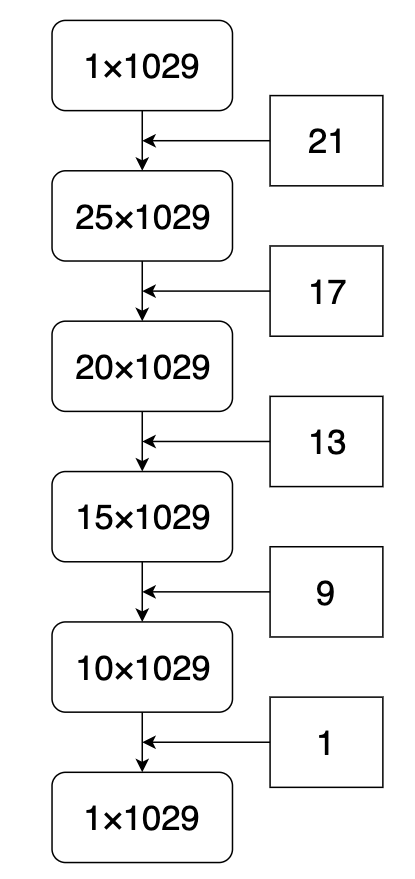
\includegraphics[width=0.8\textwidth]{img/model.png}
\end{figure}
\column{0.65\textwidth}
\lstinputlisting[language=Python, basicstyle=\tiny]{CNN}
\end{columns}
\end{frame}

\begin{frame}
\frametitle{Method 5: Training Process}
\begin{columns}
\column{0.35\textwidth}
\begin{itemize}
    \item Train CNN by each PMT Channel
    \item $\sim$450k waveform for each Channel
    \item epoch = 36
    \item Learning rate = $0.01$
\end{itemize}
\column{0.65\textwidth}
\begin{figure}
    \centering
    \caption{Loss variation during training}
    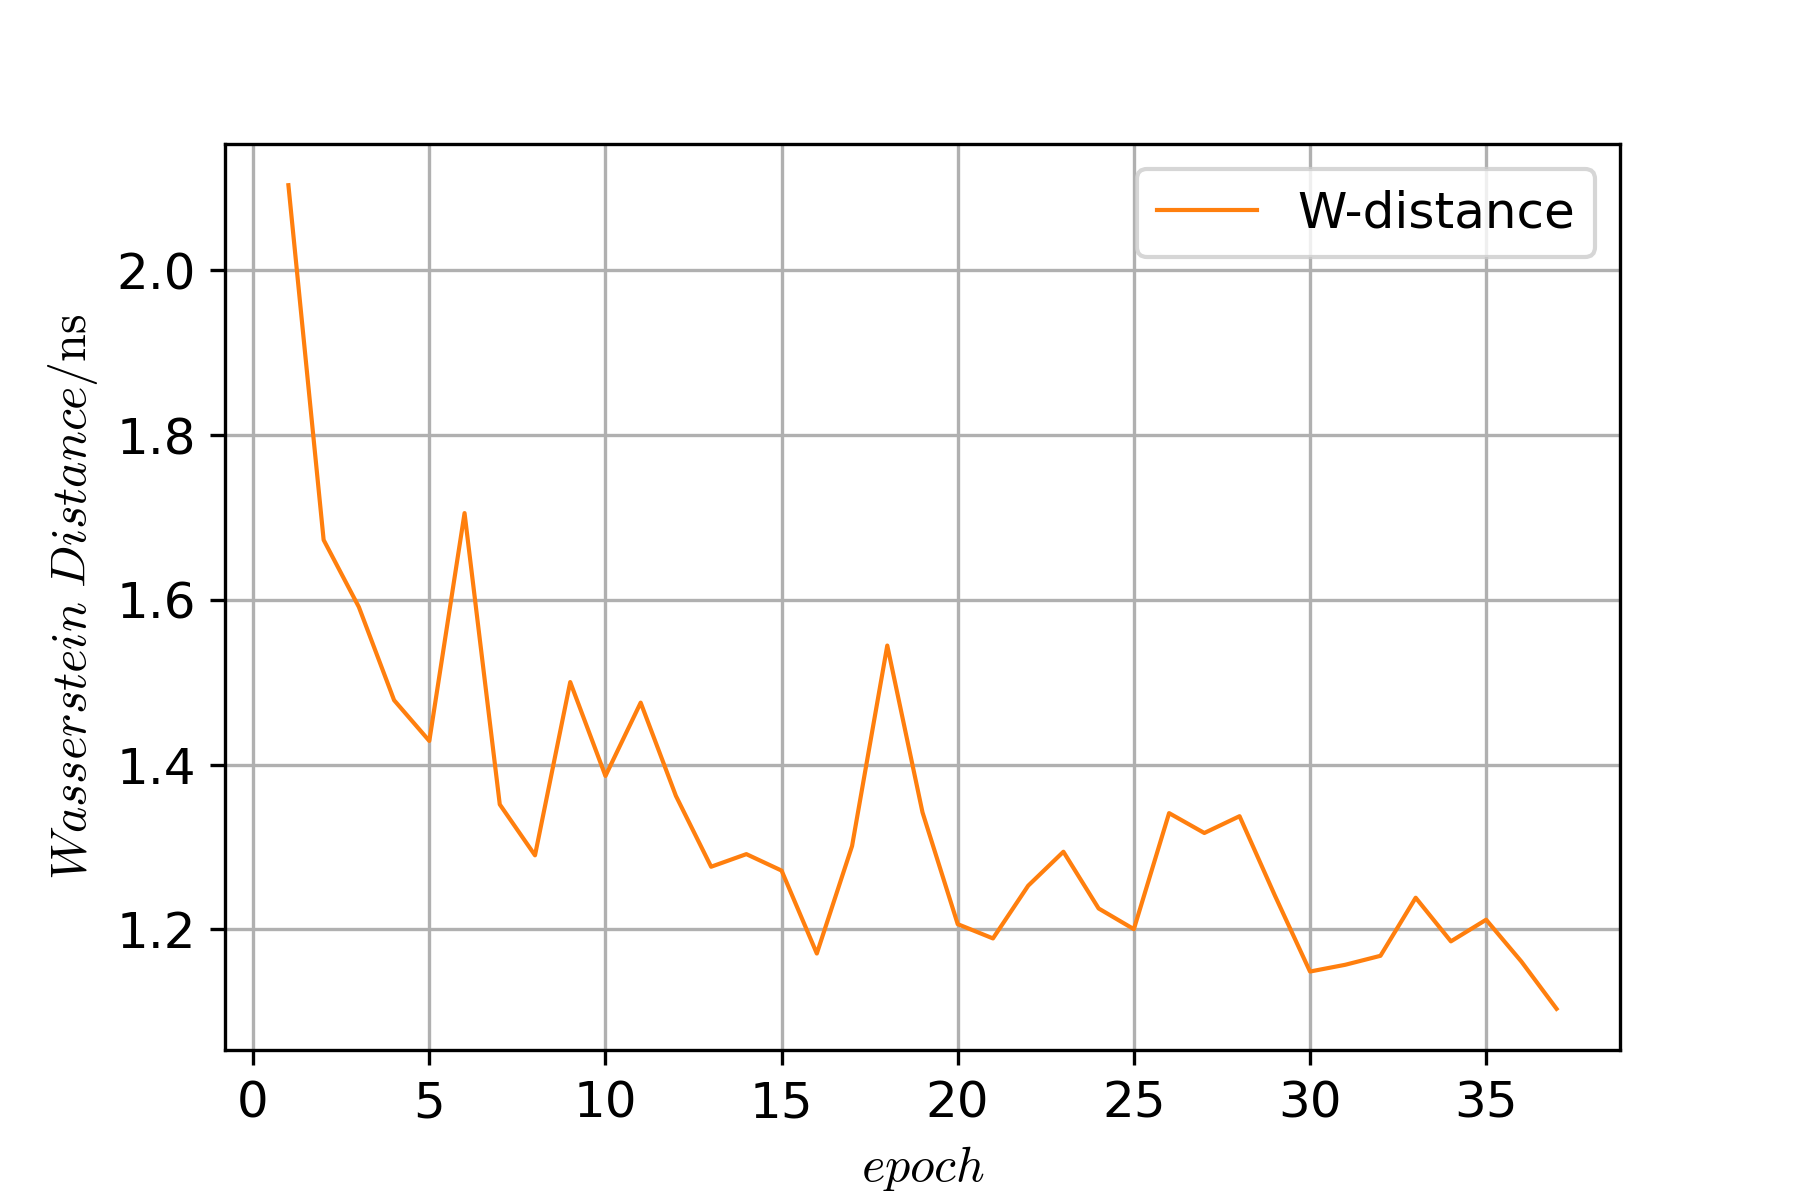
\includegraphics[width=1.0\linewidth]{img/epoch.png}
\end{figure}
\end{columns}
\end{frame}

\begin{frame}
\frametitle{Method 5: CNN Result}
\begin{figure}
    \centering
    \caption{CNN \#PE Result Histogram}
    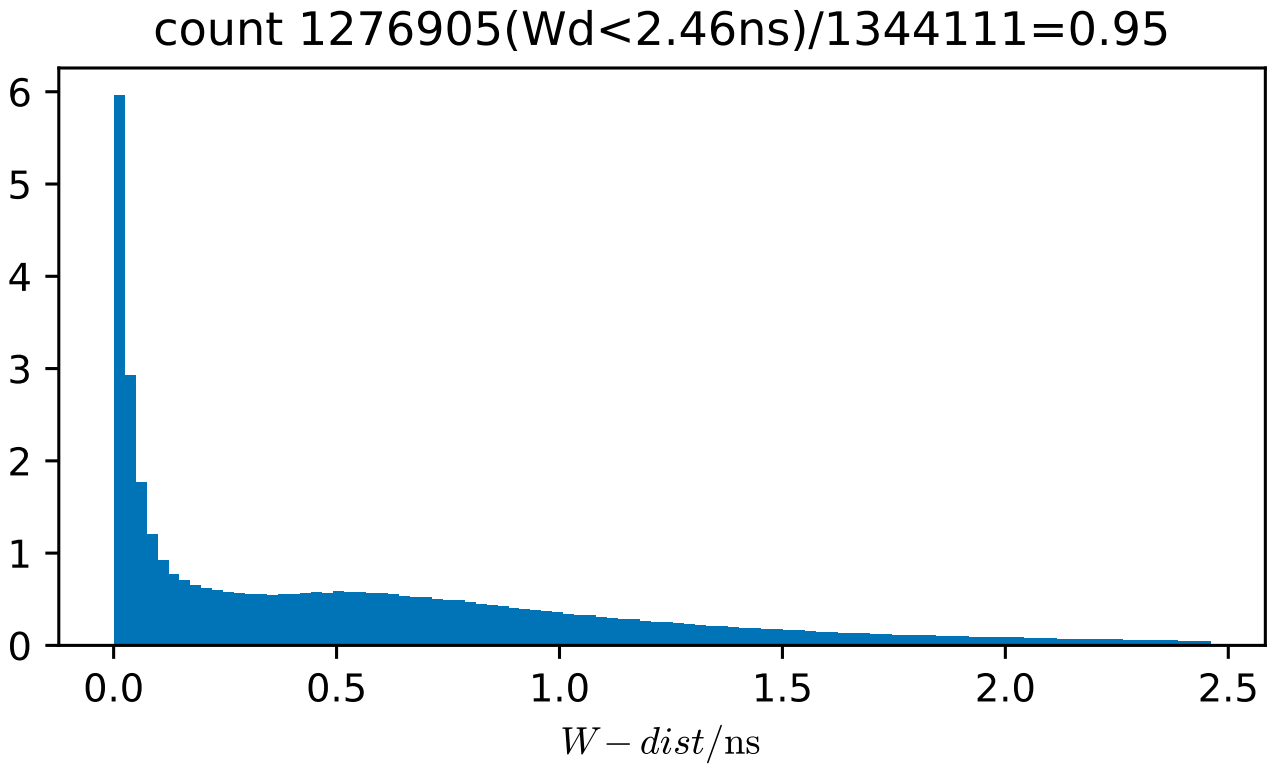
\includegraphics[width=0.85\linewidth]{img/takarapenumhist.png}
\end{figure}
\begin{center}
    Average W-dist = 2.25 (Charge), 0.76 (\#PE)
\end{center}
\end{frame}

\begin{frame}
\frametitle{Method 5: CNN Result}
\setlength{\abovecaptionskip}{0mm}
\setlength{\belowcaptionskip}{0mm}
\begin{figure}
    \centering
    \caption{CNN \#PE W-dist vs TotalPEnum}
    \includegraphics[width=0.65\linewidth]{img/takarapenumstats.png}
\end{figure}
\end{frame}

\begin{frame}
\frametitle{Method 6: Fitting (Match Pursuit) Process}
\begin{itemize}
    \item Fitting parameter: Weight in each HitTime
    \item loss is Residual sum squares of Waveform
    \item Loss = $\sum(Wave_{recon}-Wave_{truth})^{2}$
    \item using l\_bfgs\_b
\end{itemize}
\setlength{\abovecaptionskip}{0mm}
\setlength{\belowcaptionskip}{0mm}
\begin{figure}
    \centering
    \caption{Fitting Demo, W-dist = 1.51}
    \includegraphics[width=0.85\linewidth]{img/demo.png}
\end{figure}
\end{frame}

\begin{frame}
\frametitle{Method 6: Fitting Result}
\begin{figure}
    \centering
    \caption{Fitting Charge Result Histogram}
    \includegraphics[width=0.85\linewidth]{img/xiaopeipchargehist.png}
\end{figure}
\begin{center}
    Average W-dist = 0.54 (Charge), 2.46 (\#PE)
\end{center}
\end{frame}

\begin{frame}
\frametitle{Method 6: Fitting Result}
\setlength{\abovecaptionskip}{0mm}
\setlength{\belowcaptionskip}{0mm}
\begin{figure}
    \centering
    \caption{Fitting Charge W-dist vs TotalPEnum}
    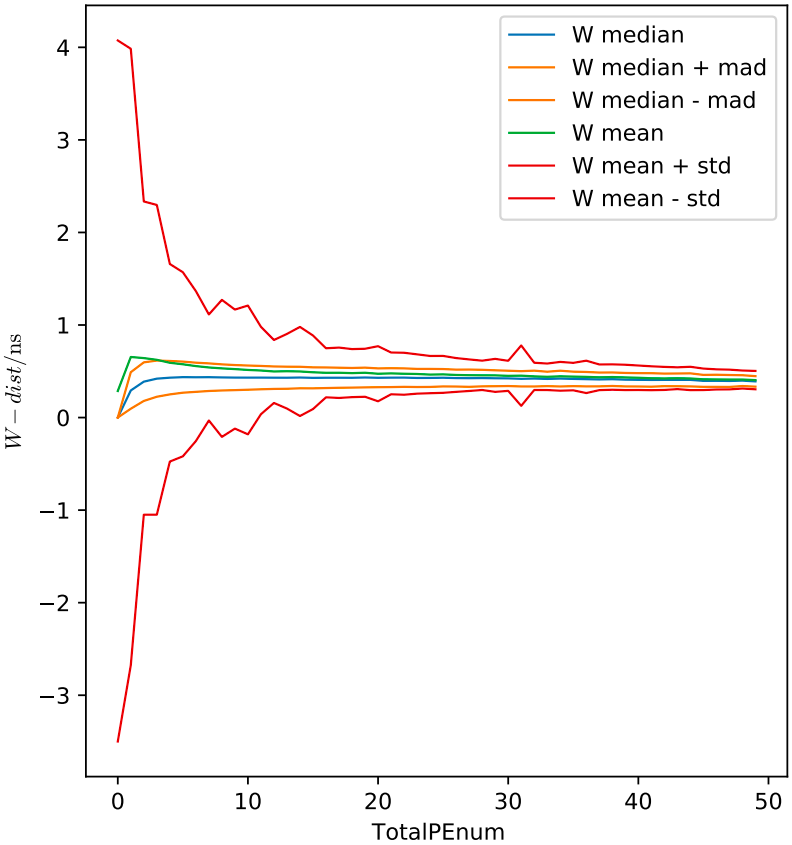
\includegraphics[width=0.65\linewidth]{img/xiaopeipchargestats-1.png}
\end{figure}
\end{frame}

\section{Result}
\begin{frame}
\frametitle{Distances}
\begin{figure}
    \centering
    \caption{Distances of methods, error bar 10 - 90 percentile (Charge)}
    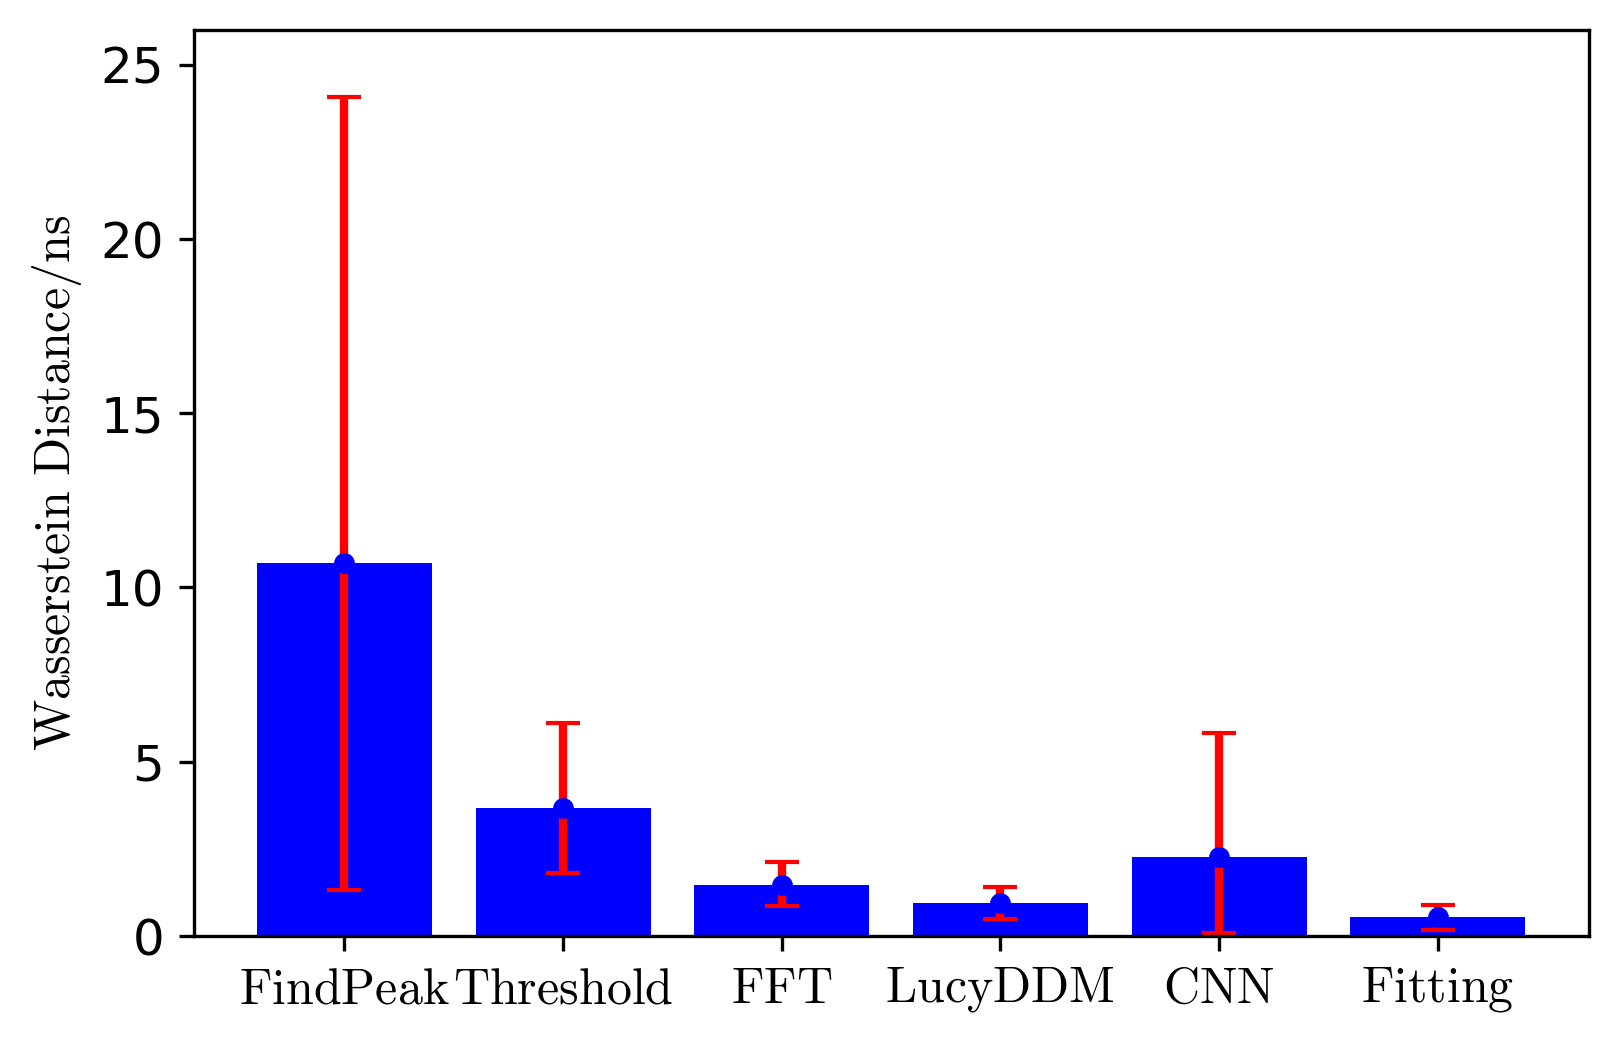
\includegraphics[width=1.0\linewidth]{img/summarycharge.png}
\end{figure}
\end{frame}

\begin{frame}
\frametitle{Distances}
\begin{figure}
    \centering
    \caption{Distances of methods, error bar 10 - 90 percentile (\#PE)}
    \includegraphics[width=1.0\linewidth]{img/summarypenum.png}
\end{figure}
\end{frame}

\begin{frame}
\frametitle{Efficiency}
\begin{table}
    \centering
    \caption{Reconstruction Efficiency}
    \begin{tabular}{c|c|c}
        \hline
        &  & Performance \\
        \hline
        CNN & Charge & 6.0s/$10^{5}$Wf (gpu) \\
        \hline
        CNN & \#PE & 6.0s/$10^{5}$Wf (gpu)\\
        \hline
        Fitting & Charge & 2000s/$10^{5}$Wf (cpu) \\
        \hline
        Fitting & \#PE & 2000s/$10^{5}$Wf (cpu) \\
        \hline
        LucyDDM & Charge & 24s/$10^{5}$Wf (cpu) \\
        \hline
        LucyDDM & \#PE & 24s/$10^{5}$Wf (cpu) \\
        \hline
    \end{tabular}
\end{table}
\hspace{4mm}\begin{itemize}
    \item gpu: Using half of NVIDIA Tesla K80
    \item cpu: Using 50 CPU core of AMD EYPC 7702
\end{itemize}
\end{frame}

\section{Summary \& Outlook}
\begin{frame}
\frametitle{Summary \& Outlook}
\begin{itemize}
    \item We developed several representative methods to extract photon timing information hidden in PMT waveform. 
    \item These methods will improve event reconstruction and particle identification. 
    \item We are working on applying these methods to event reconstruction and particle identification. 
    \item Fitting method is the best for reconstruction of Charge, while LucyDDM looks promising. 
    \item CNN method is the best for reconstruction of \#PE. 
\end{itemize}
\end{frame}

\begin{frame}
\frametitle{Acknowledgement}
\begin{itemize}
    \item Prof. Shaomin Chen \& Prof. Zhe Wang, Tsinghua University, Jinping Neutrino Experiment Collaboration
    \item Developer of JSAP(Jinping neutrino experiment Simulation and Analysis Package), Ziyi Guo et al. 
    \item Aiqiang Zhang \& Jihui Pei, Tsinghua University
    \item Student Association of Science and Technology, Department of Engineering Physics, Tsinghua University
    \item Student Association of Science and Technology, Department of Physics, Tsinghua University
    \item Student Association of Science and Technology, Department of Computer Science and Technology, Tsinghua University
\end{itemize}
\end{frame}

\appendix
\section{Backup}
\begin{frame}[noframenumbering]
\thispagestyle{empty}
\frametitle{Backup - Poisson Distance \& Charge Diff}
\hspace{4mm}Poisson Distance is used \textbf{only} when reconstruct \#PE
\begin{itemize}
    \item $Q = \sum \#PE_{truth_i}; q = \sum \#PE_{recon_i}$
    \item $D_{p} = |Q-q|*\mathrm{Poisson}(Q|Q)$
\end{itemize}
\hspace{4mm}Charge Diff is used \textbf{only} when reconstruct Charge
\end{frame}

\begin{frame}[noframenumbering]
\thispagestyle{empty}
\frametitle{Backup - TotalPEpos vs TotalPEnum}
\begin{columns}
\column{0.5\textwidth}
\begin{figure}
    \centering
    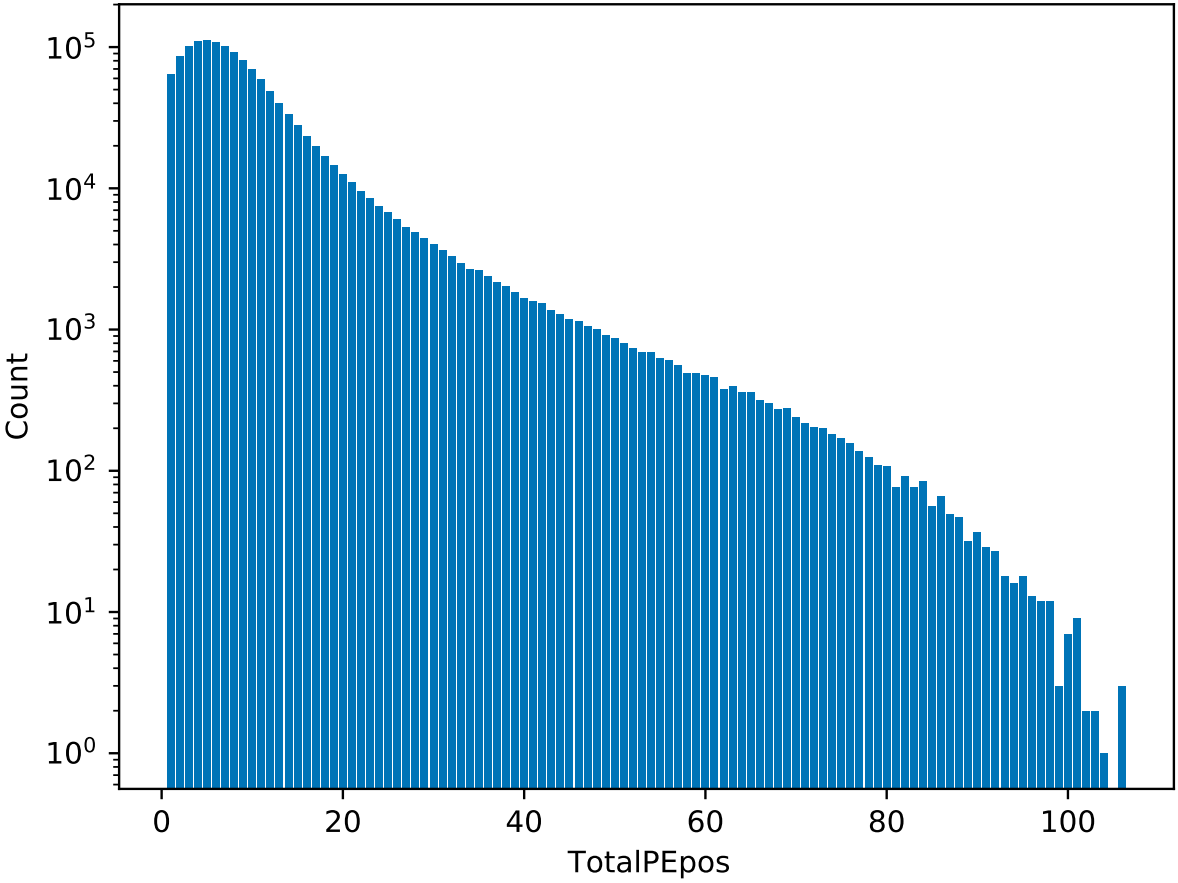
\includegraphics[width=1.0\linewidth]{img/pepos.png}
\end{figure}
\column{0.5\textwidth}
\begin{figure}
    \centering
    \includegraphics[width=1.0\linewidth]{img/penum.png}
\end{figure}
\end{columns}
\end{frame}

\begin{frame}[noframenumbering]
\thispagestyle{empty}
\frametitle{Backup - Fitting Result}
\begin{figure}
    \centering
    \caption{Fitting \#PE Result Histogram}
    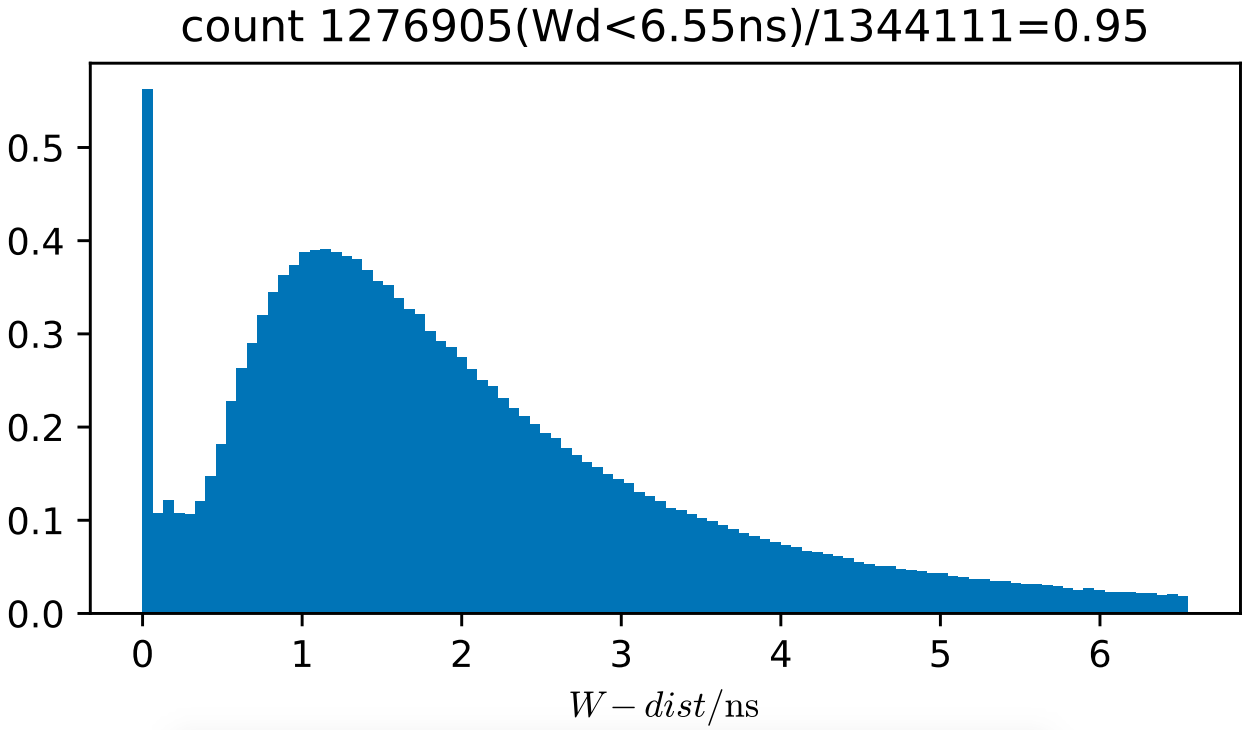
\includegraphics[width=0.85\linewidth]{img/xiaopeippenumhist.png}
\end{figure}
\end{frame}

\begin{frame}[noframenumbering]
\thispagestyle{empty}
\frametitle{Backup - Fitting Result}
\setlength{\abovecaptionskip}{0mm}
\setlength{\belowcaptionskip}{0mm}
\begin{figure}
    \centering
    \caption{Fitting \#PE W-dist vs PEpos}
    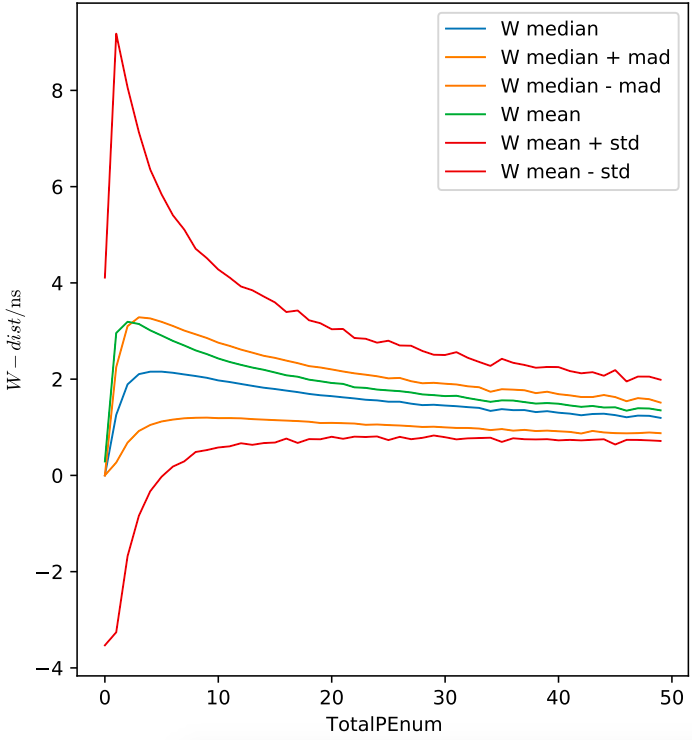
\includegraphics[width=0.65\linewidth]{img/xiaopeippenumstats.png}
\end{figure}
\end{frame}

\begin{frame}[noframenumbering]
\thispagestyle{empty}
\frametitle{Backup - CNN Result}
\begin{figure}
    \centering
    \caption{CNN Charge Result Histogram}
    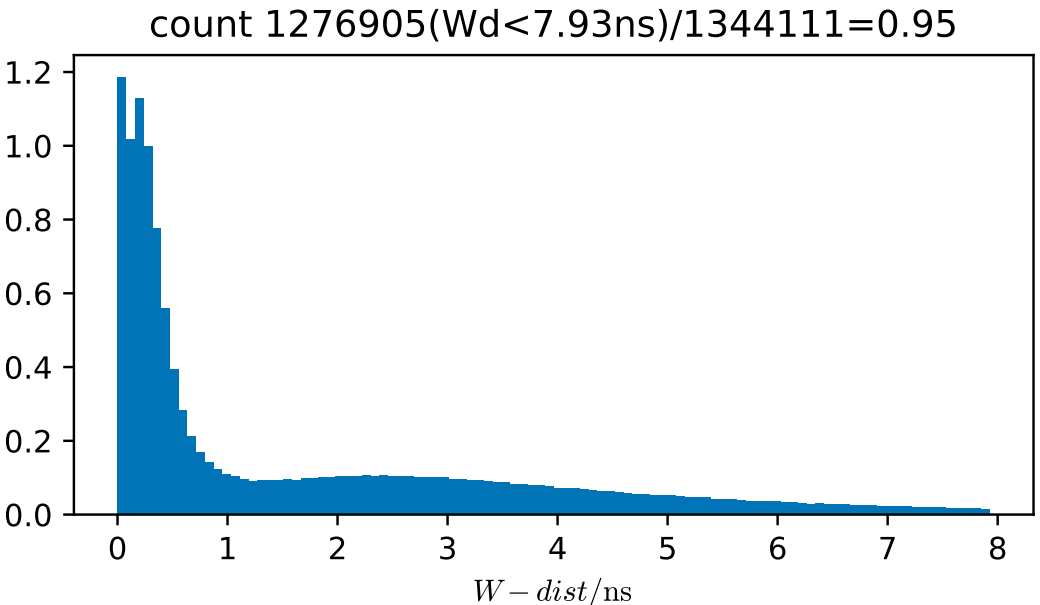
\includegraphics[width=0.85\linewidth]{img/takarachargehist.png}
\end{figure}
\end{frame}

\begin{frame}[noframenumbering]
\thispagestyle{empty}
\frametitle{Backup - CNN Result}
\setlength{\abovecaptionskip}{0mm}
\setlength{\belowcaptionskip}{0mm}
\begin{figure}
    \centering
    \caption{CNN Charge W-dist vs PEpos}
    \includegraphics[width=0.65\linewidth]{img/takarachargestats.png}
\end{figure}
\end{frame}

\begin{frame}[noframenumbering]
\thispagestyle{empty}
\frametitle{Backup - Large W-dist}
\begin{figure}
    \centering
    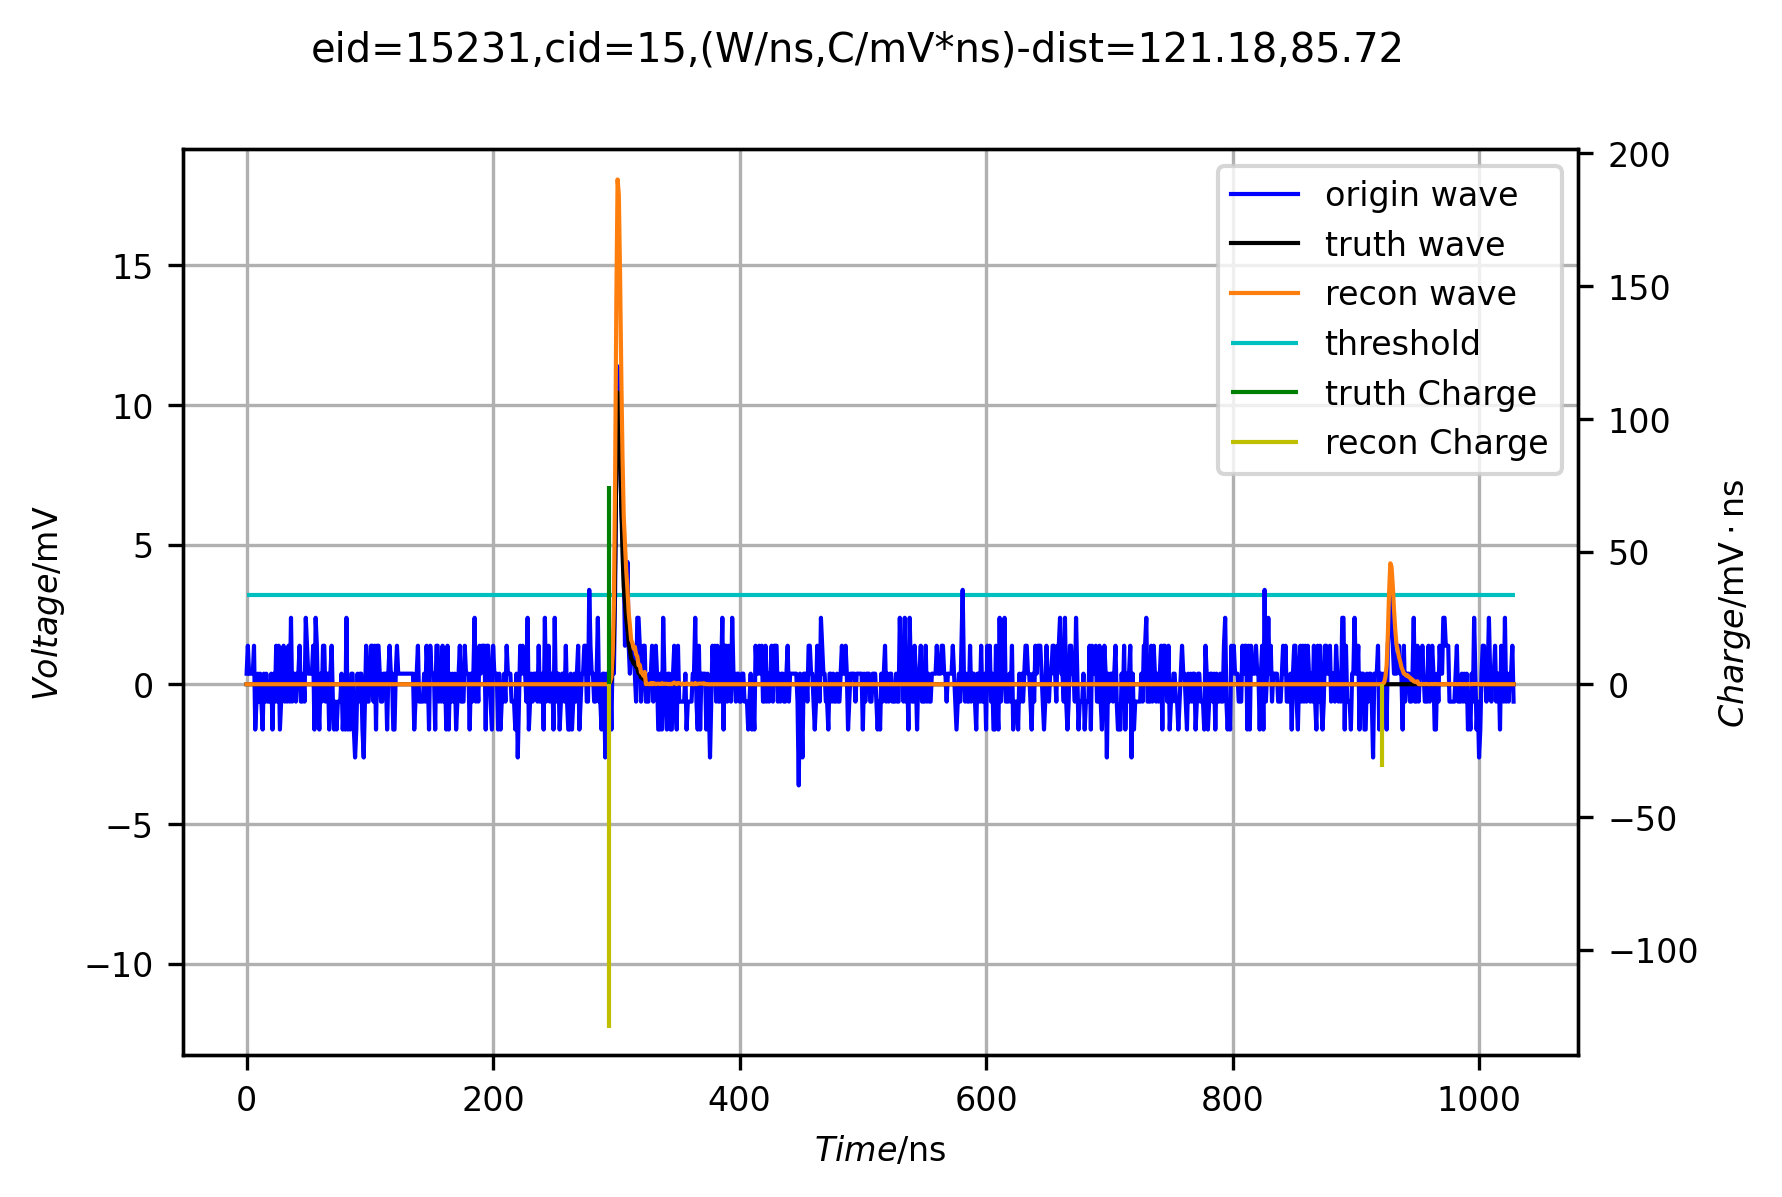
\includegraphics[width=1.0\linewidth]{img/demoe15231c15.png}
\end{figure}
\end{frame}

\begin{frame}[noframenumbering]
\thispagestyle{empty}
\frametitle{Backup - Large W-dist}
\begin{figure}
    \centering
    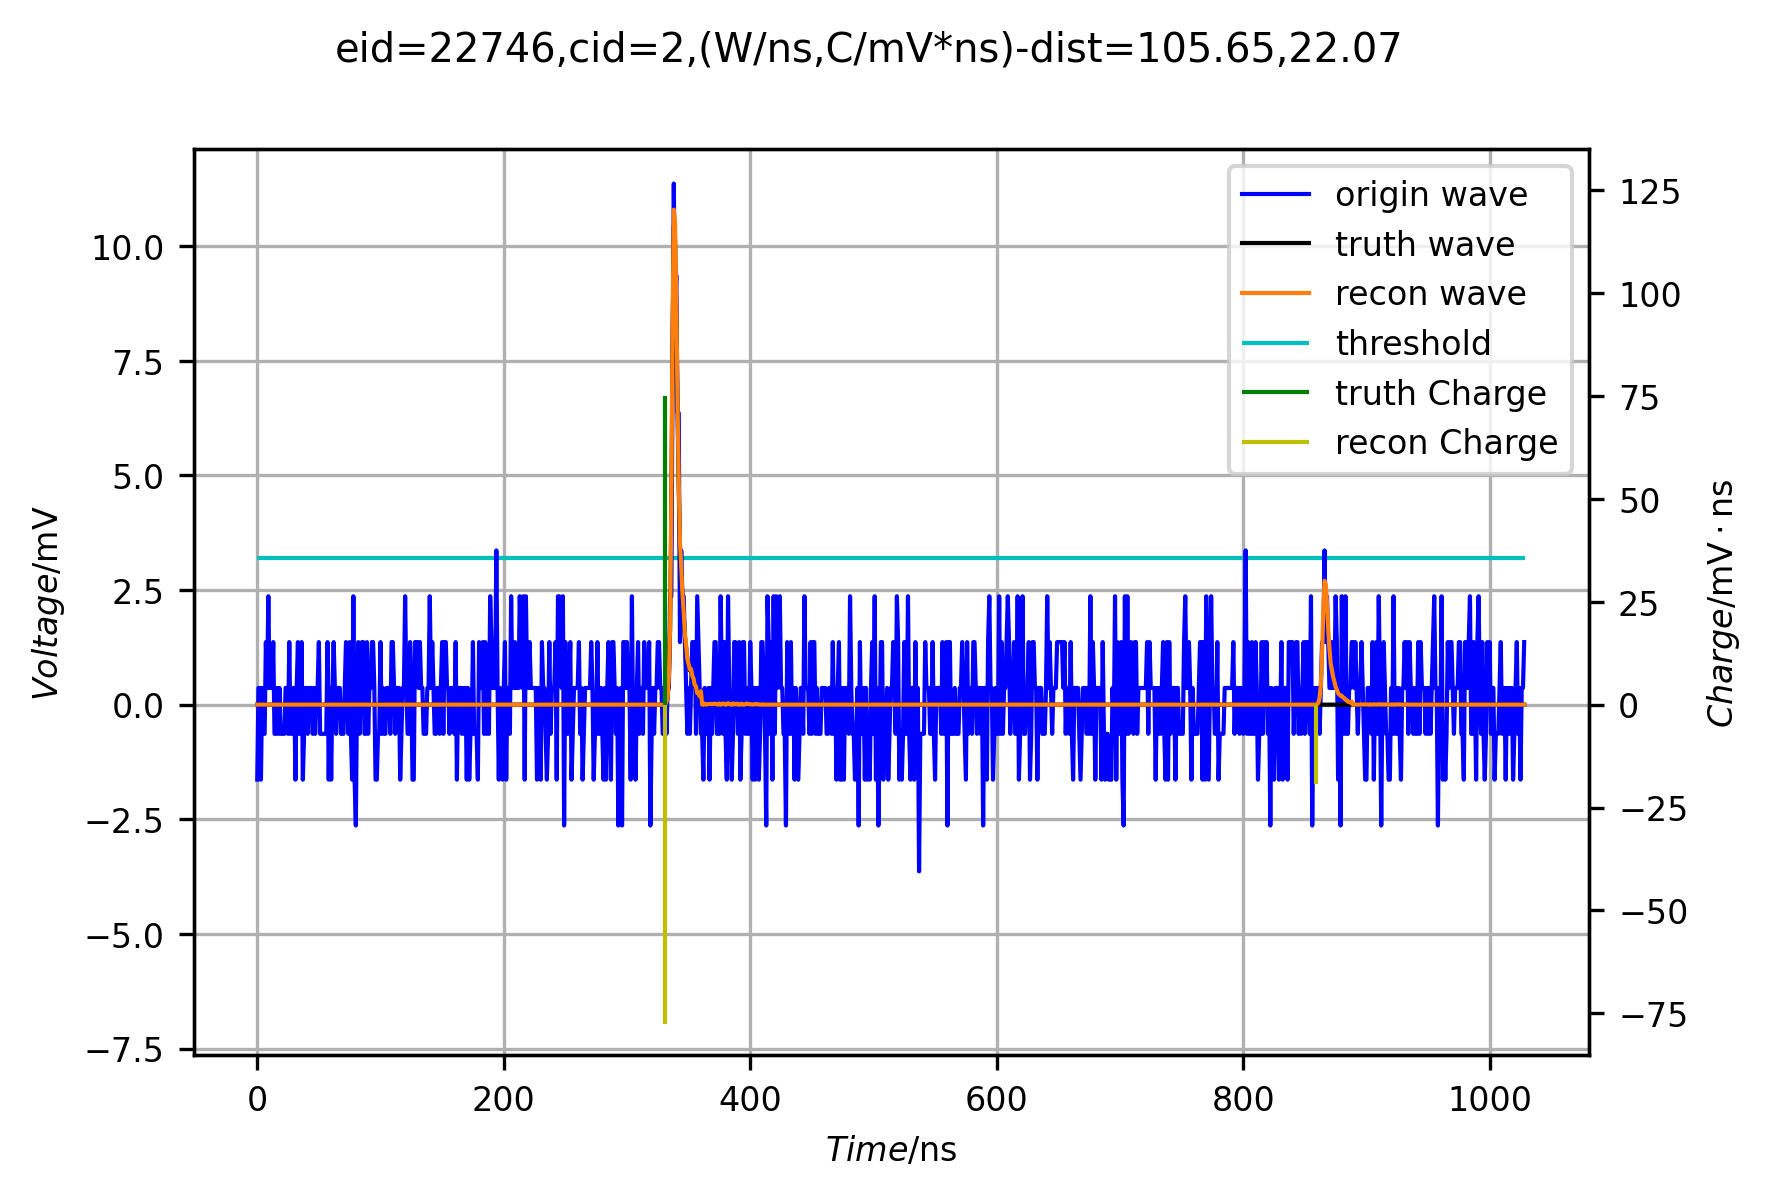
\includegraphics[width=1.0\linewidth]{img/demoe22746c2.png}
\end{figure}
\end{frame}

\end{document}